

\section{Technologies}

\subsection{Frontend}
% Three languages can be used to implement the frontend while using one of the main popular frameworks. This consists of i) JavaScript \cite{javascript}, ii) TypeScript \cite{typescript} and iii) Scala.js \cite{scalajs}. We decided to avoid JavaScript due to the lack of type support. Between TypeScript and Scala.js, we ended up choosing TypeScript over Scala.js. That is because we are more familiar with TypeScript than Scala.js. Moreover, the advantages of Scala.js, according to their website \cite{scalajs}, do not provide much more facilities than what TypeScript has already done. Therefore, TypeScript is selected as our main language to implement the frontend.

% With regard to the frontend framework, there were three frameworks that we considered. Unlike the main language, we are familiar with all three frameworks. Angular \cite{angular} is a large framework with extensive pre-built tools and libraries. However, we decided not to use Angular, because this would have made our frontend unnecessarily large.

% Vue.js \cite{vue} is another popular framework with a large community similar to React \cite{react}. However, Vue.js is not as widely used as React, according to the number of available repository results on GitHub \cite{reactsearch, vuesearch}. That means React has a bigger community that we can rely on. Hence, we decided to use React as our frontend framework.

% According to the concept design \cite{checklistdesign}, the frontend consists of four main screens as follows: \vspace{-8pt}
% Three frontend programming languages to be considered includes: i) JavaScript \cite{javascript}, ii) TypeScript \cite{typescript}, and iii) Scala.js \cite{scalajs}. Although JavaScript and TypeScript are identical in virtually every way, JavaScript does not support static typing. Therefore, we decided to remove JavaScript from the list due to the absence of type support. Scala.js was added to the list because WorkflowFM was using Scala as the backend programming language. However, due to the lack of expertise with Scala.js, we decided to stick with what we were familiar with, which was TypeScript.

TypeScript \cite{typescript} was selected as the programming language for the frontend. That was because we were familiar with TypeScript and its frameworks. 
Although JavaScript \cite{javascript} and TypeScript are identical in virtually every way, JavaScript does not support static typing. Static typing is important to detect potential bugs or errors in the codebase. That was another reason that we chose TypeScript over other languages.

Next.js \cite{nextjs} was chosen as the frontend framework. Next.js is a framework on top of React \cite{react}, a widely used frontend framework, and improves upon it. For the fact that React has the biggest community among frontend frameworks, being React-based would help us if we get stuck somewhere during the implementation.

% Even though the programming language had been decided, we had to select the framework for the prototype. There were three frameworks to be considered: i) Angular \cite{angular}, ii) Nuxt.js (Vue) \cite{nuxtjs, vue}, and iii) Next.js (React) \cite{nextjs, react}. In the end, we decided to use Next.js, which is a framework on top of React, because React has the biggest community among the three, which would be convenient if we get stuck somewhere with the framework.

As Next.js was chosen, Redux \cite{redux} was automatically determined as the state management tool. Redux is centralised storage for all components in an application specifically made for React library.

Finally, we had to decide on the CSS framework among various options. Since we prioritised the flexibility in CSS customisation, we chose TailwindCSS \cite{tailwindcss} as the CSS framework for this project. In contrast to other frameworks, TailwindCSS only offers pre-built classes, not components. This gave us the customisation we wanted.

\subsection{Backend}
The backend programming language was decided to be Scala \cite{scala} because WorkflowFM's execution engine was also using Scala. Using the same language would make the integration between our system and WorkflowFM easier.

As for the framework, we originally planned to use http4s \cite{http4s}. However, due to some technical issues, we could not deploy a http4s project to a cloud service for a quick test in the beginning. Thus, we migrated the framework to Akka-http \cite{akka}. After a quick deployment, Akka-http worked perfectly fine. That is why we chose Akka-http as our backend framework.

% The language that we select to implement the backend of the project is Scala. The reason that we choose Scala over other languages is that WorkflowFM's execution engine is currently using Scala. Hence, using the same language will make it easier to integrate with the execution engine.

% Http4s \cite{http4s} is selected as the framework for the backend. This is because we decide to use RESTful \cite{richardson2008restful} as the protocol to communicate between the server and the client. In fact, there were multiple options that we were considering. However, each of them does not suit well with what we want to do.\vspace{-8pt}

% \begin{itemize}
%     \item Vertx \cite{vertx} is a large framework and has multiple variations in JVM languages. And because of that, Vertx is unnecessary large and not specifically built for functional programming compared to other frameworks.
%     \item Cask \cite{cask} is a microframework. However, Cask is still very young and is not widely used compared to other frameworks. Considering that we are new to Scala, we decided to use other frameworks to avoid unexpected circumstances.
%     \item Akka \cite{akka} is very similar to http4s in terms of community and library size. However, http4s has slightly bigger community than Akka's. Therefore, we decided to use http4s instead.
%     % due to the lack of details in Akka's documentation, we decided to use http4s instead.
% \end{itemize}

% \vspace{-8pt}Therefore, http4s is chosen because it is the most suitable framework compared to other alternatives.


\subsection{Database}
% PostgreSQL was our choice as the database of the system because i) it is a relational database
Originally, we planned to use SQLite \cite{sqlite} as the database since Chen's healthcare database was provided in SQLite. However, the majority of service providers did not offer strong support for SQLite. Because we intended to host the entire project online, we chose to switch the database to PostgreSQL \cite{postgresql}. PostgreSQL is a relational database, much like SQLite, but it is widely used by many developers and has tons of support from cloud providers. This will be helpful if we ever migrate our database later on.
We decided to use PostgreSQL as a service called ElephantSQL \cite{elephantsql} because our prototype was still in the minimum viable product (MVP) stage and could use the service in its free tier.


\subsection{Continuous Integration and Continuous Deployment (CI/CD)}

Since we hosted our codebase on GitHub \cite{github}, it was simple to use GitHub Actions \cite{githubactions} as the continuous integration of our project. As for the continuous deployment, we hosted the frontend on Vercel \cite{vercel} and the backend on Heroku \cite{heroku}, which both provided the continuous deployment service integrated into GitHub.

% \begin{itemize}
%     \item Miscellaneous
%     \begin{itemize}
%         \item GitHub
%         \item GitHub Actions
%         \item PostgreSQL
%         \item ElephantSQL
%         \item Vercel
%         \item Heroku
%     \end{itemize}
% \end{itemize}

% - choices: React, Vue, Angular, Scala.js

% - chose: React, Next.js, TailwindCSS, Redux

% - choices: Node.js, Scala, Java

% - choices for Scala: akka-http, http4s, play

% chose: Scala, Akka-http

% - GitHub, GitHub Actions, PostgreSQL, ElephantSQL, Vercel, Heroku


\section{Frontend}
The implementation of the frontend was based on Design sections \ref{design:software_structure} and \ref{interface_design}. The routing was divided based on section \ref{design:software_structure}, while the navigation and interfaces were based on section \ref{interface_design}.
This prototype is hosted online and can be accessed through \href{https://resource-based-checklist-generation.vercel.app/}{HERE}.

\subsection{Landing}
\label{im:landing}

As mentioned in Design sections \ref{design:software_structure}, this is the main screen of this web application. The navigation from the main screen to the canvas screen follows the navigation in Design section \ref{interface_design}.
It connects the canvas screen (\ref{im:canvas_screen}) through the \verb!Create a New Template! button in the middle-top of the screen, as shown in Figure \ref{fig:main_screen}, following with the process selection popup (Figure \ref{fig:process_input}) and the auto-generation popup (Figure \ref{fig:autogen}).
% The bottom section is a list of saved checklist templates. Each template
Furthermore, this screen allows users to access the view checklist screen (\ref{im:view_checklist}) through selecting a template in the list of saved checklist templates in the bottom section.
% The main screen requires the connection to Backend's Checklist, according to Design section \ref{design:software_structure}, because it needs to display a list of saved checklist templates as shown in the bottom section of Figure \ref{fig:main_screen}.

% call template creation on the popup, 
% call auto generation on the popup
\begin{figure}[ht!]
    \centering
    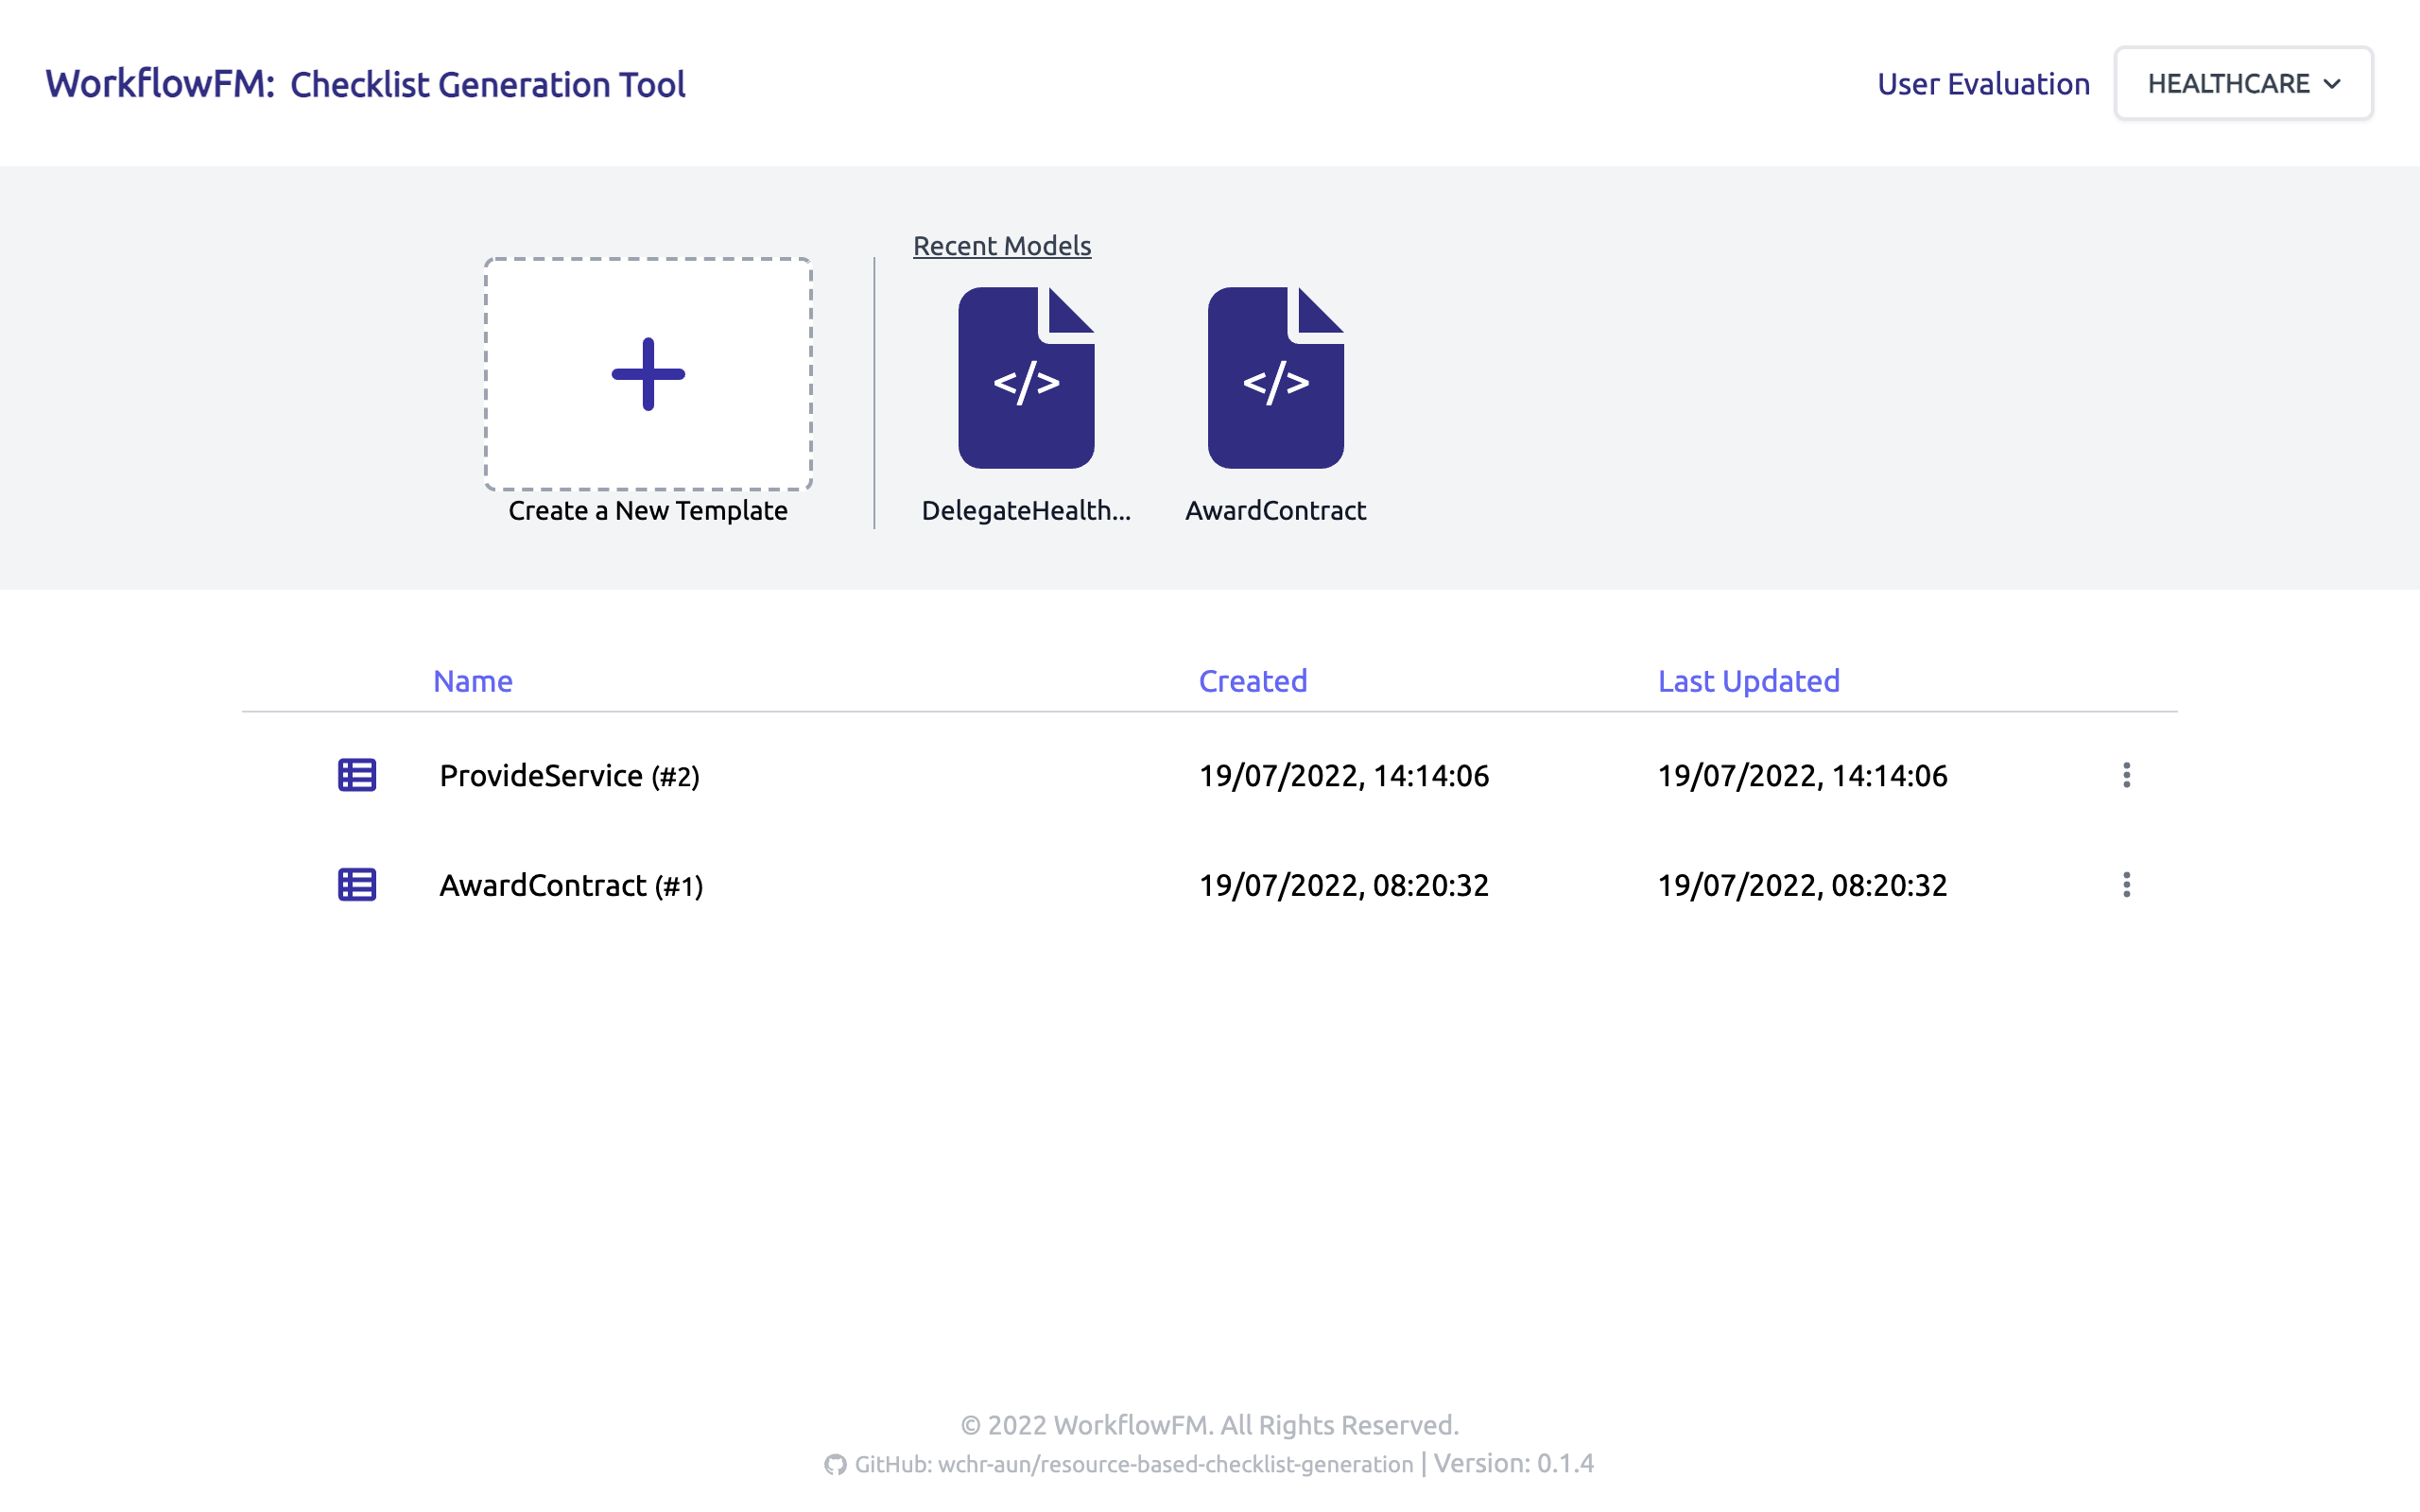
\includegraphics[width=0.6\textwidth]{overleaf/images/screens/main_screen.png}
    \caption{Main Screen}
    \label{fig:main_screen}
\end{figure}


\begin{figure}[ht!]
\centering
\begin{minipage}{.5\textwidth}
  \centering
  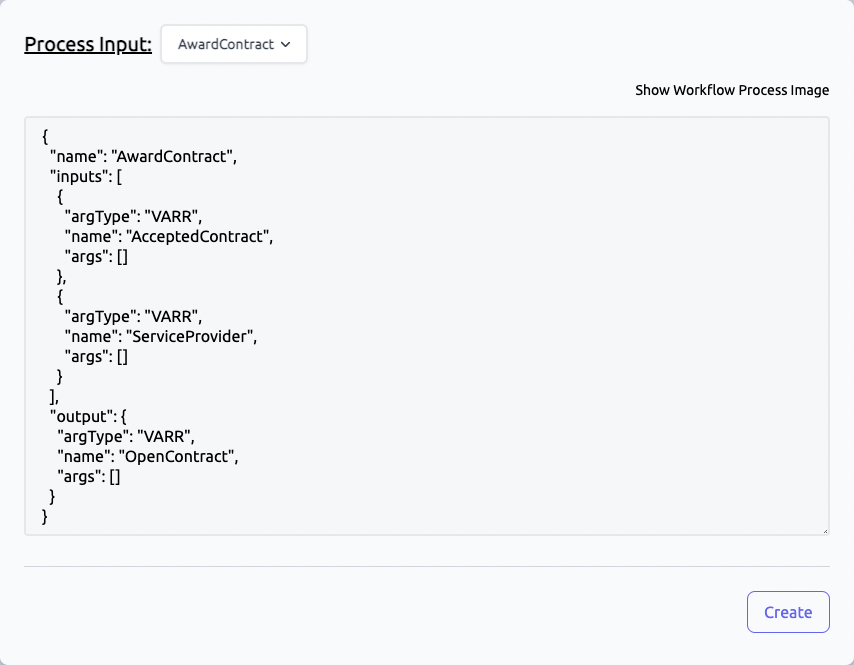
\includegraphics[width=0.9\linewidth]{overleaf/images/screens/process_input.png}
  \caption{Select Process Popup}
  \label{fig:process_input}
\end{minipage}%
\begin{minipage}{.5\textwidth}
  \centering
  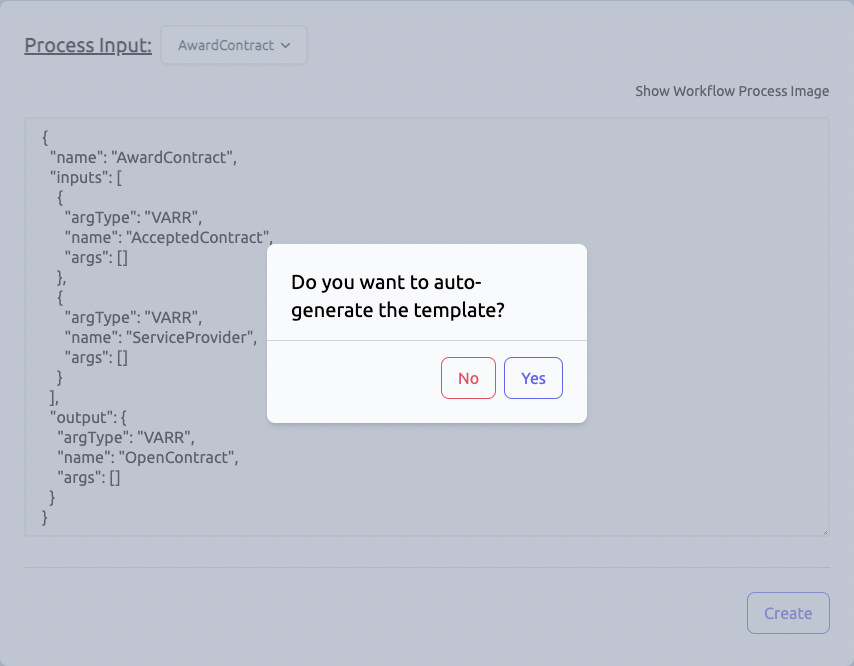
\includegraphics[width=0.9\linewidth]{overleaf/images/screens/autogen.png}
  \caption{Auto-Generation Popup}
  \label{fig:autogen}
\end{minipage}
\end{figure}




\subsection{Canvas}
\label{im:canvas}

In this section, we implemented three screens: Canvas Screen, Dependencies Management Popup, and Preview Screen. Similarly to section \ref{im:landing}, we followed the navigation between these screens from section \ref{interface_design} in Design.


% input information query here,
% query recommendation here,
% template saving here

\subsubsection{Canvas Screen}
\label{im:canvas_screen}

% This screen covers five functionalities, according to the software's structure section \ref{design:software_structure}: Template Creation, Input Information Query, Form Adjustment, Template Saving, and Query Recommendation.
% mention what this screen covers functionalities

As seen in Figure \ref{fig:canvas_screen}, the canvas screen contains three sections: checklist’s name, input information, and form adjustment. These sections are implemented following the checklist template's structure in section \ref{checklist_strcuture}. The display name of each section can be edited. Other than the display names, the input information and the form adjustment sections can adjust the sequence order of what appears before or after as well as the visibility of each field, as shown in Figures \ref{fig:input_information_section} and \ref{fig:form_section}.

% \begin{figure}[ht!]
%     \centering
%     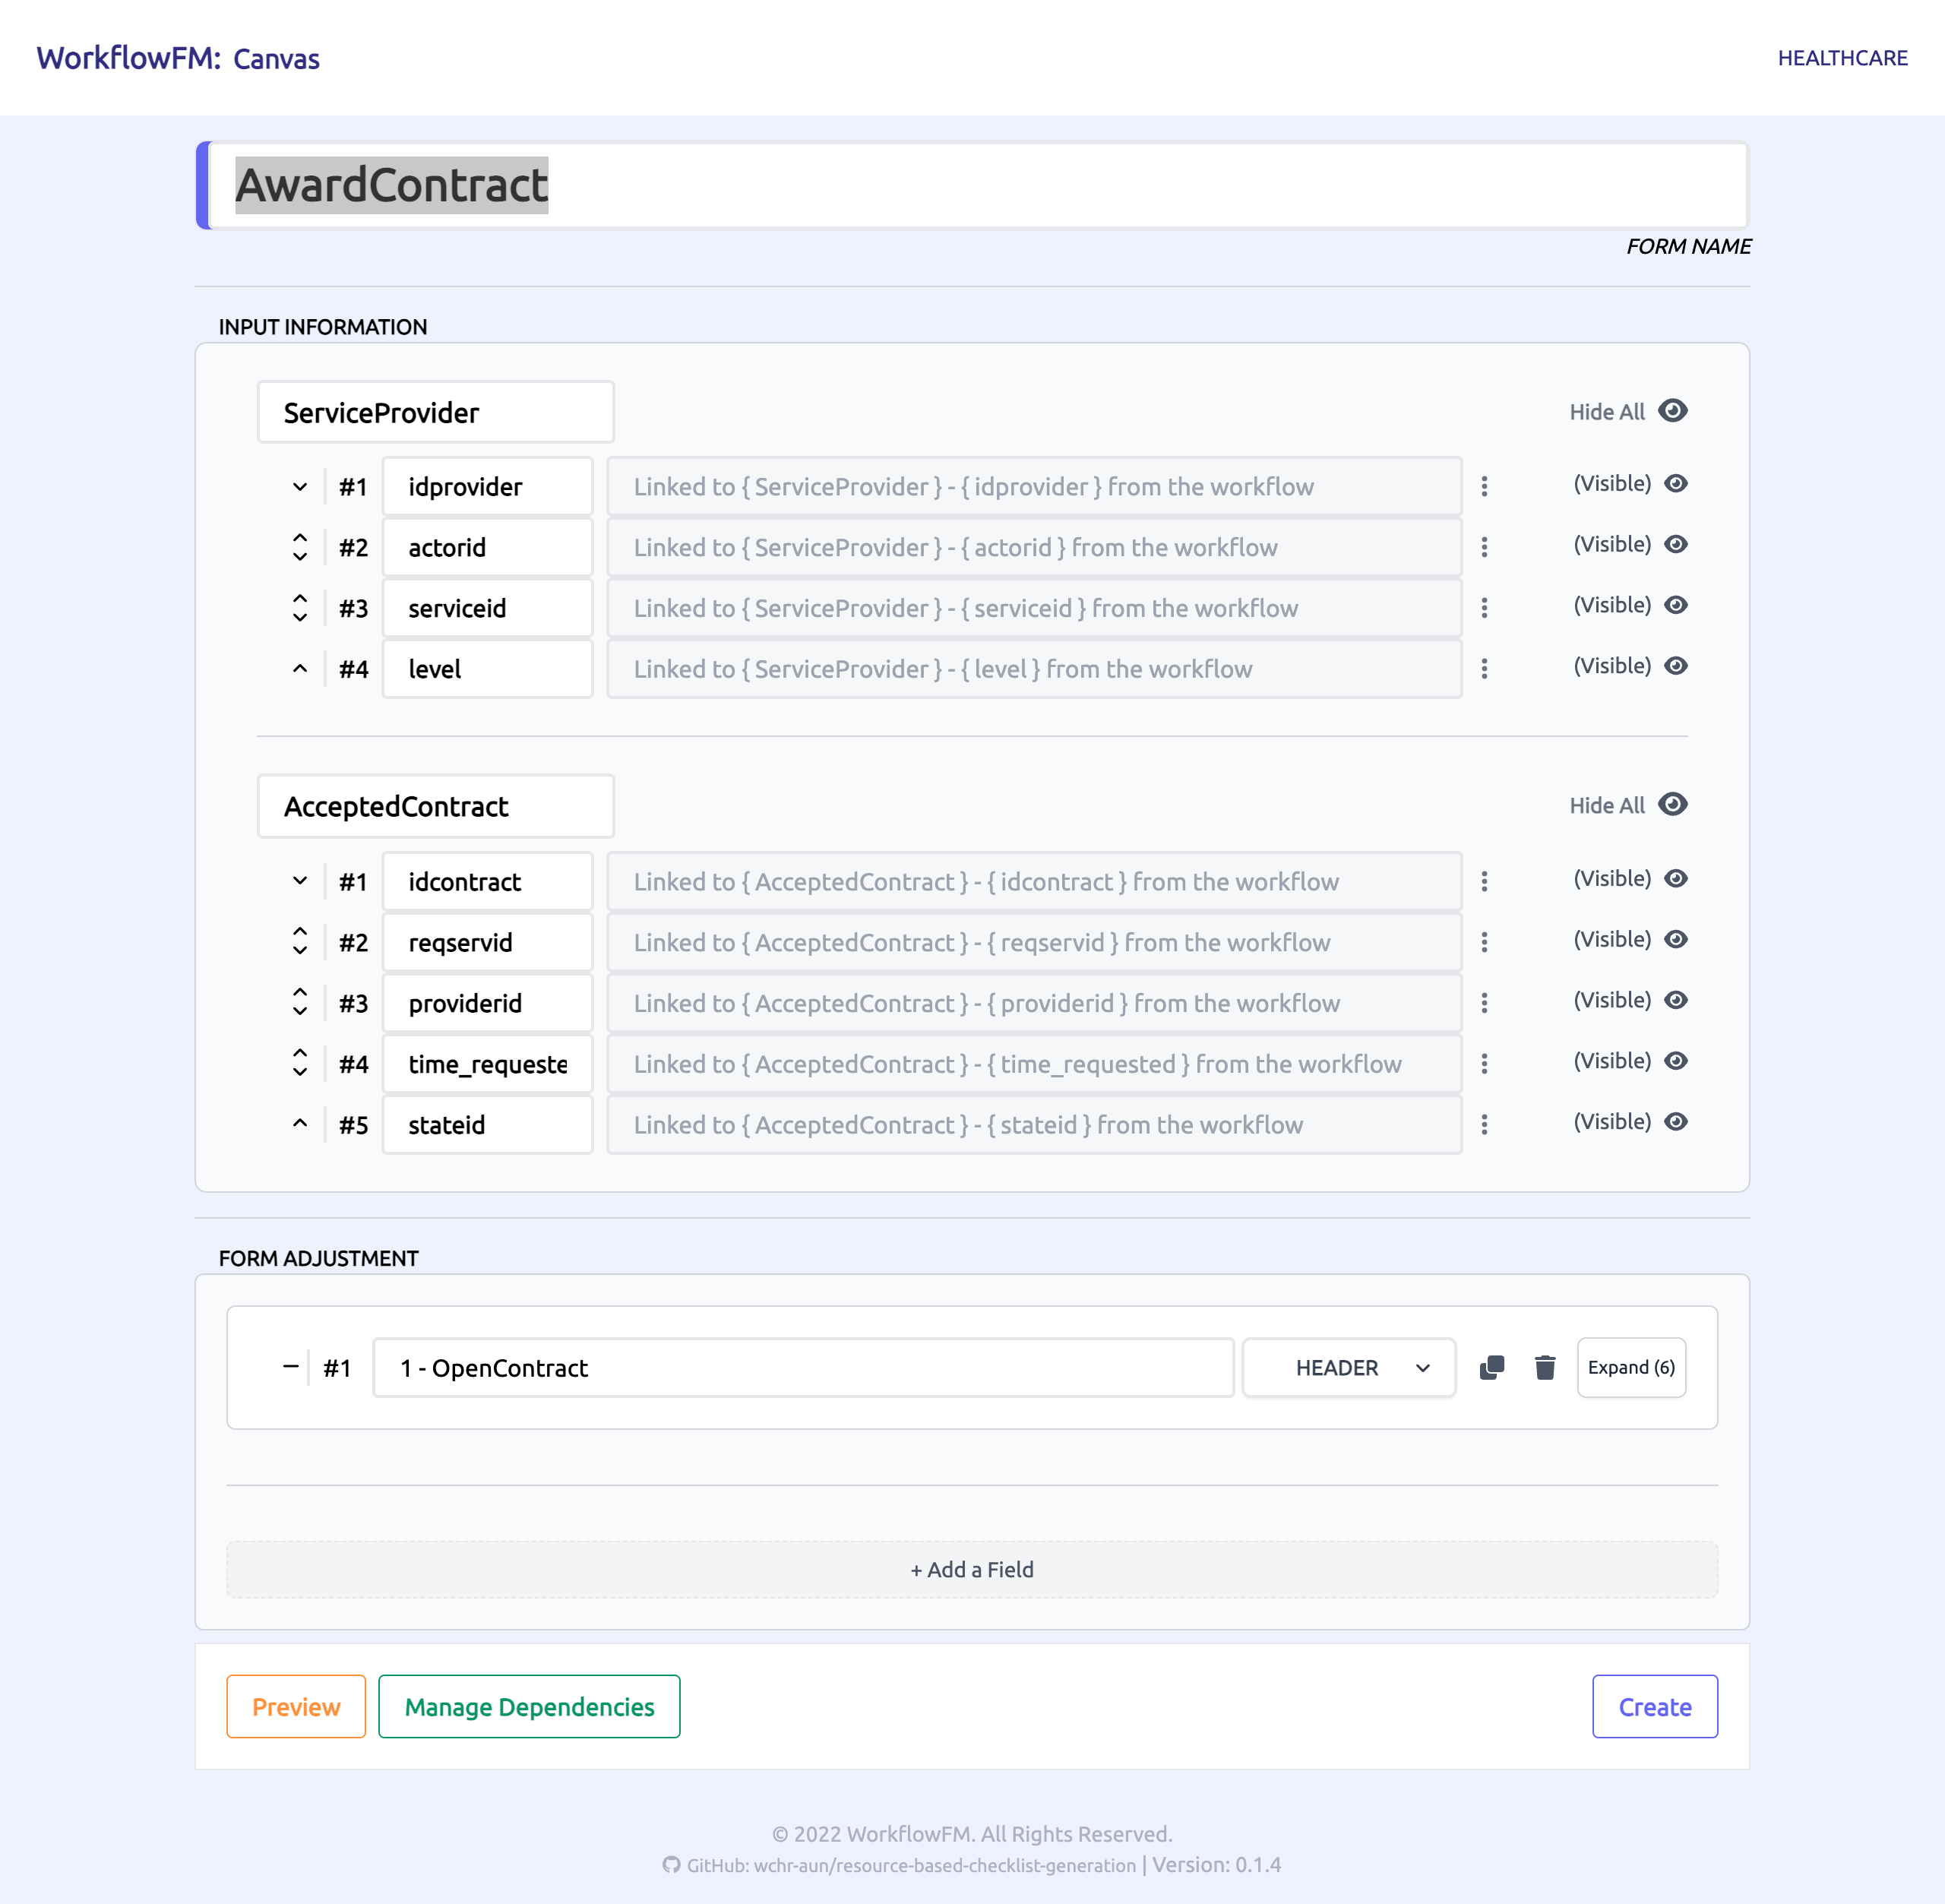
\includegraphics[width=0.6\textwidth]{overleaf/images/screens/canvas_screen.png}
%     \caption{Canvas Screen}
%     \label{fig:canvas_screen}
% \end{figure}

% form adjustment here
Designers can change the component type and the requirability of a component in the form adjustment section. There are ten component types: header, tab, textbox, paragraph, dropdown, choices, checkboxes, date, time, and constant. In addition, a new component can be added via the button at the bottom of each component. This all together is the \textbf{Form Adjustment} functionality.

\begin{figure}[ht!]
\centering
\begin{minipage}{.5\textwidth}
  \centering
  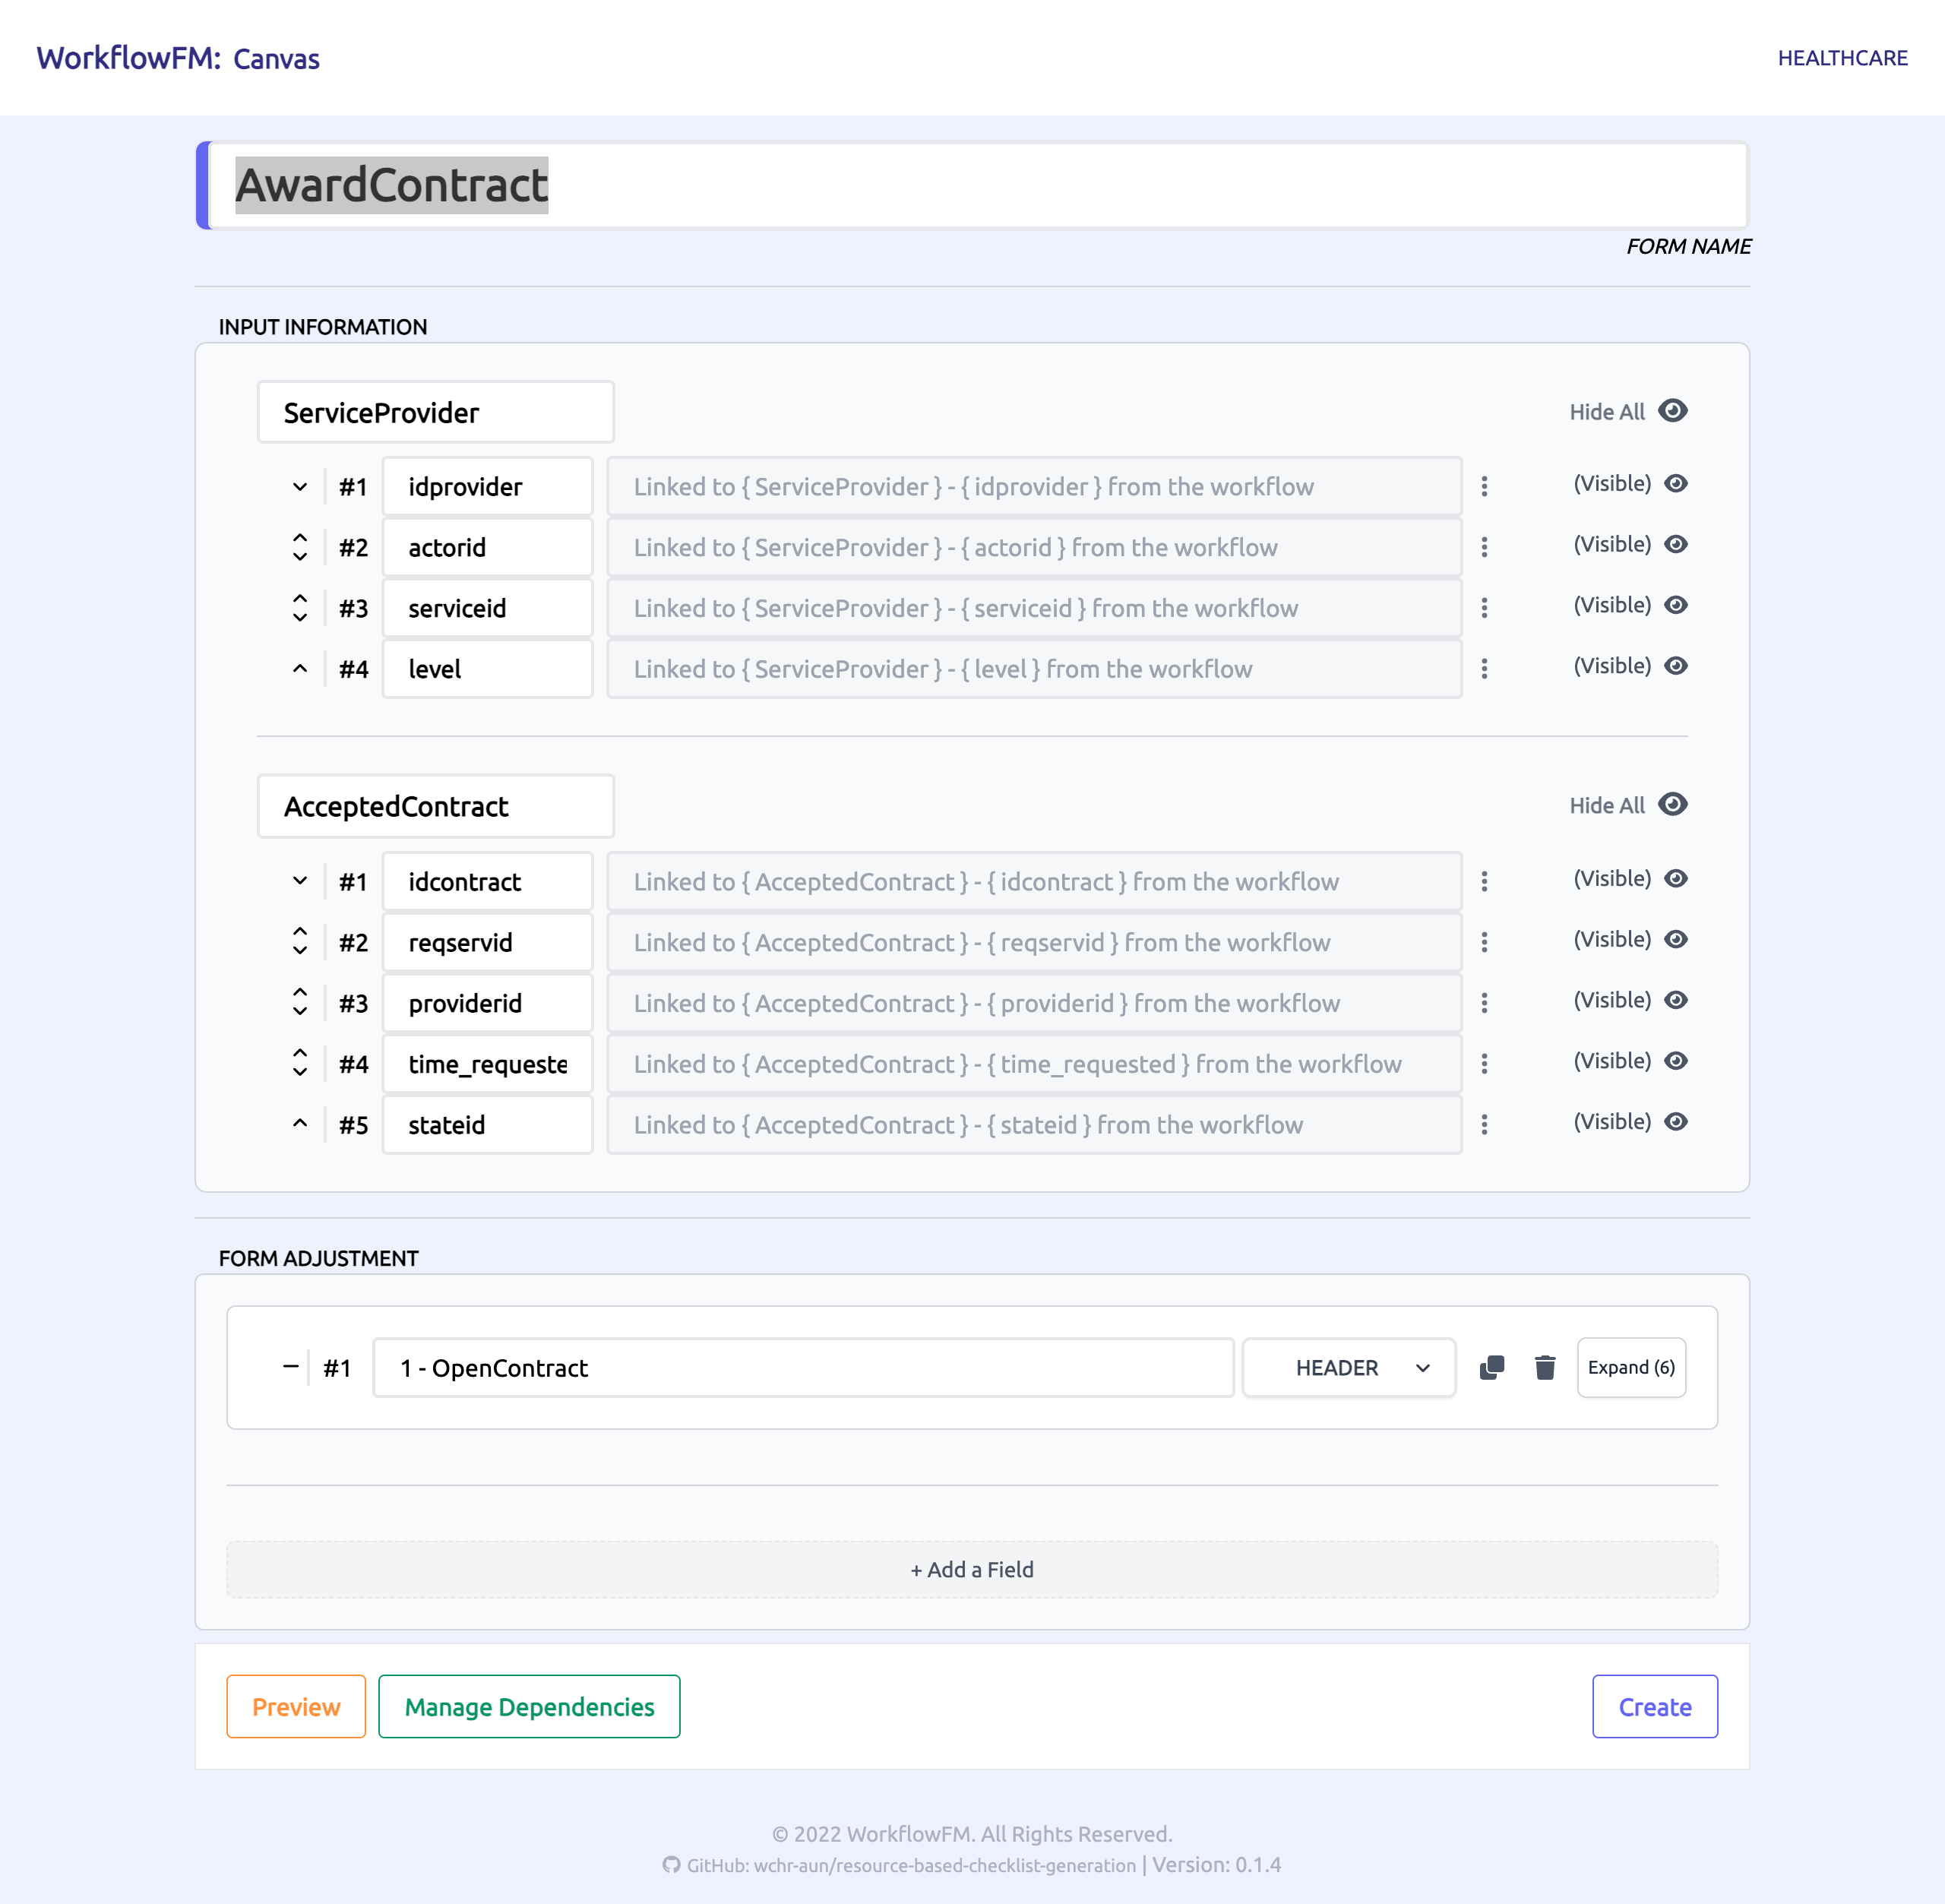
\includegraphics[width=0.9\linewidth]{overleaf/images/screens/canvas_screen.png}
  \caption{Canvas Screen}
  \label{fig:canvas_screen}
\end{minipage}%
\begin{minipage}{.5\textwidth}
  \centering
  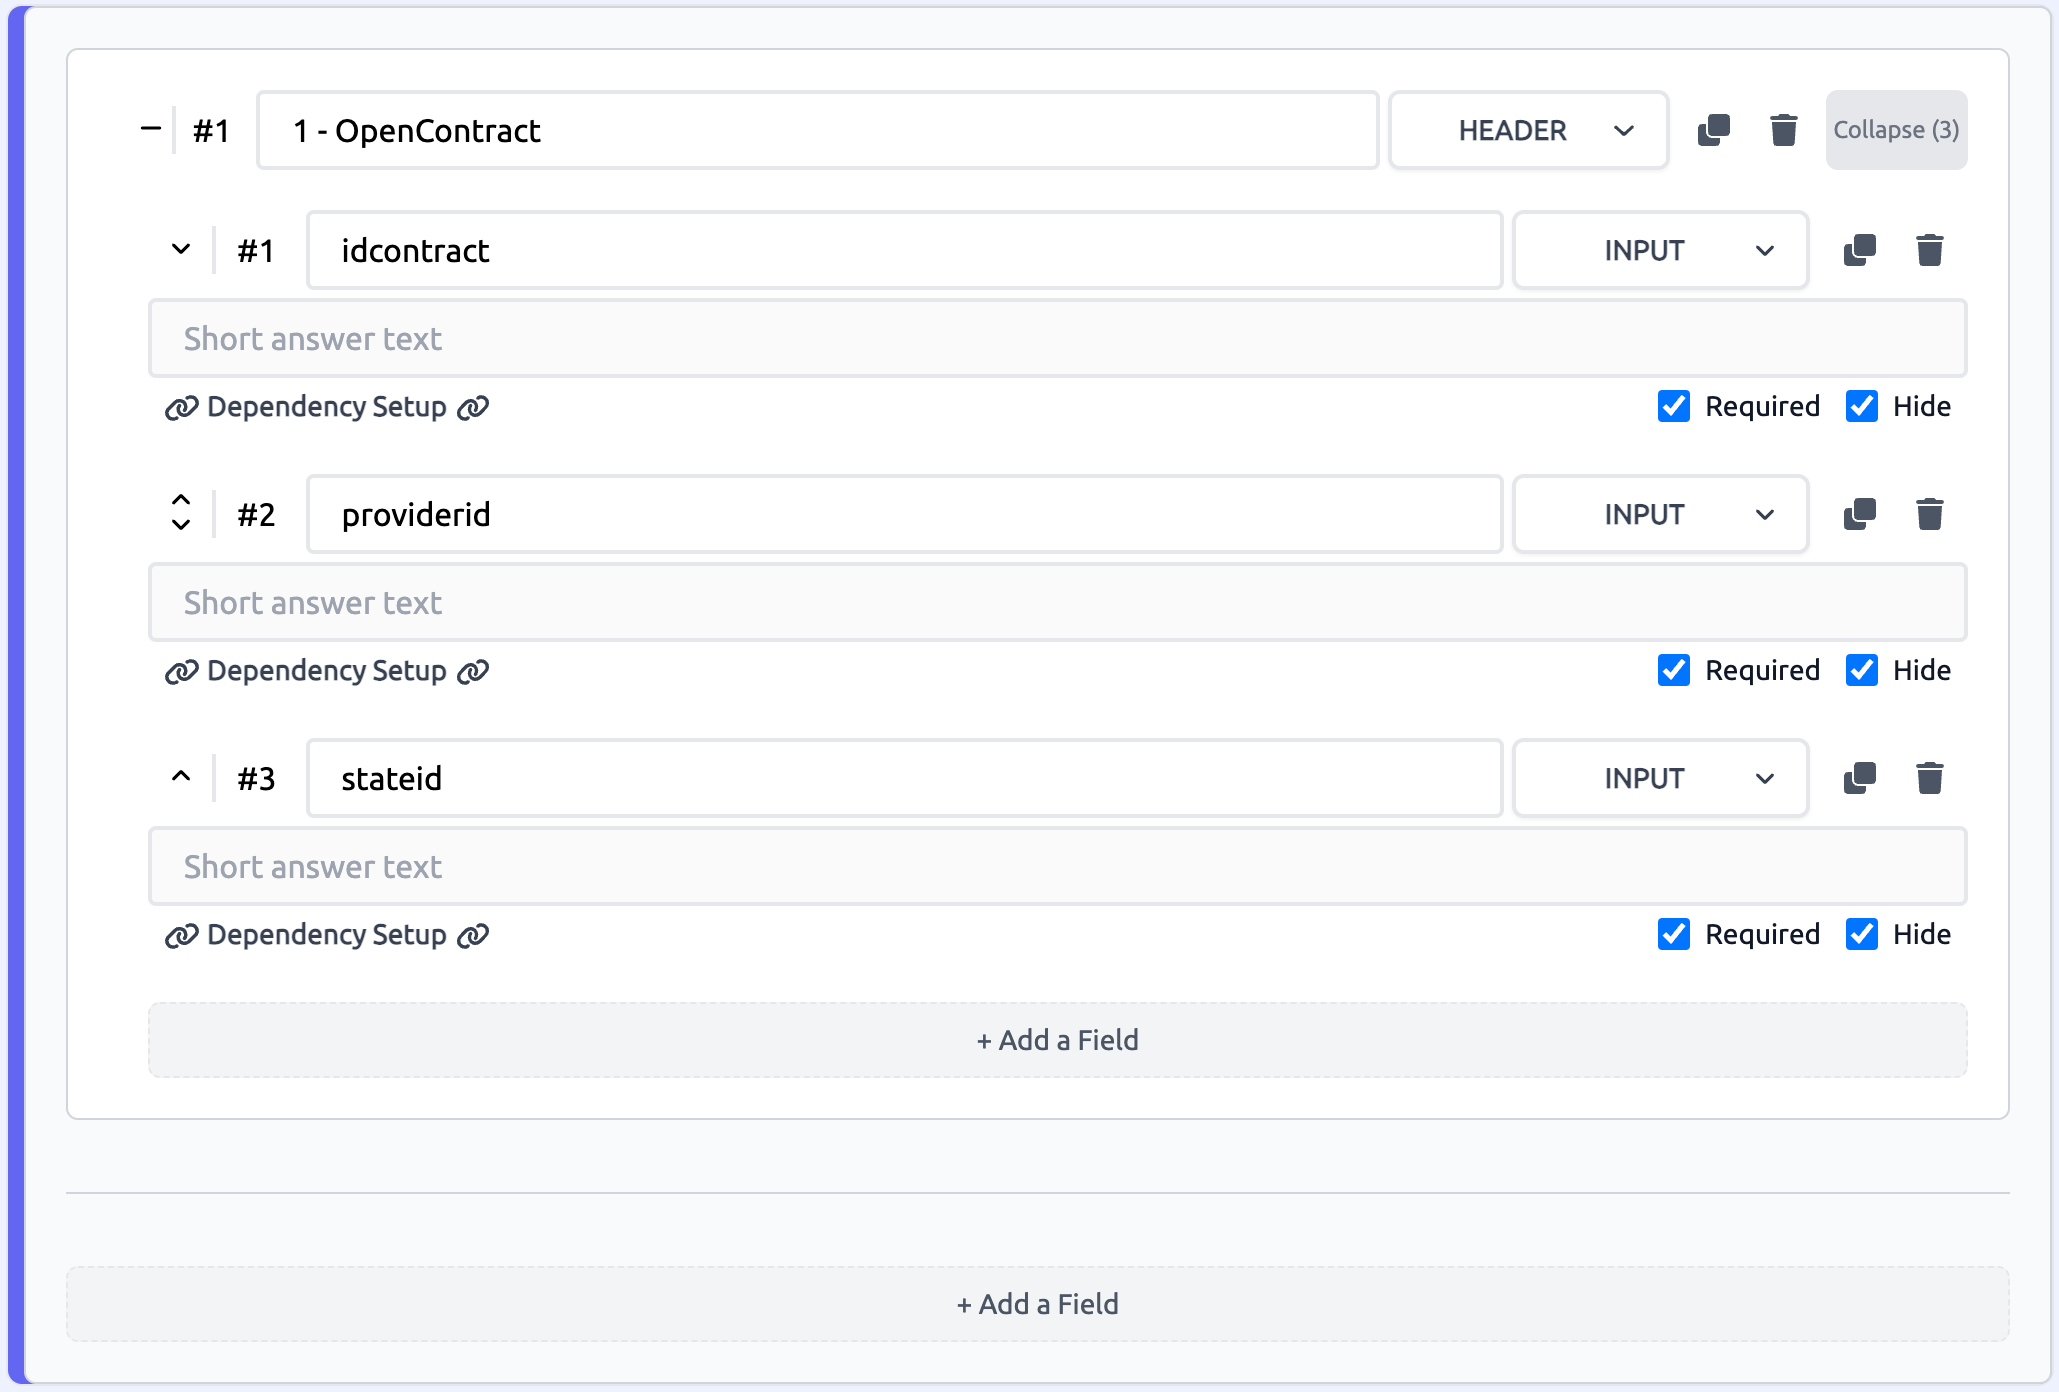
\includegraphics[width=0.9\linewidth]{overleaf/images/screens/form_section.png}
  \caption{Form Section}
  \label{fig:form_section}
\end{minipage}
\end{figure}


% Additional parts of the input infromation section
Additional to the input information section, new input information fields can be added through either ``Query more information using this field" or ``Get suggested query input information" options inside the vertical ellipsis icon (\vdots) in Figure \ref{fig:input_information_section}. This is the \textbf{Input Information Query} function. Selecting ``Get suggested query input information" will call the \textbf{Query Suggestion} function and display all the suggested fields, as shown in \ref{fig:query_suggestion}. Both the \textbf{Input Information Query} function and the \textbf{Query Suggestion} functionalities will be further elaborated in section \ref{backend_dependency}




\begin{figure}[ht!]
\centering
\begin{minipage}{.5\textwidth}
  \centering
  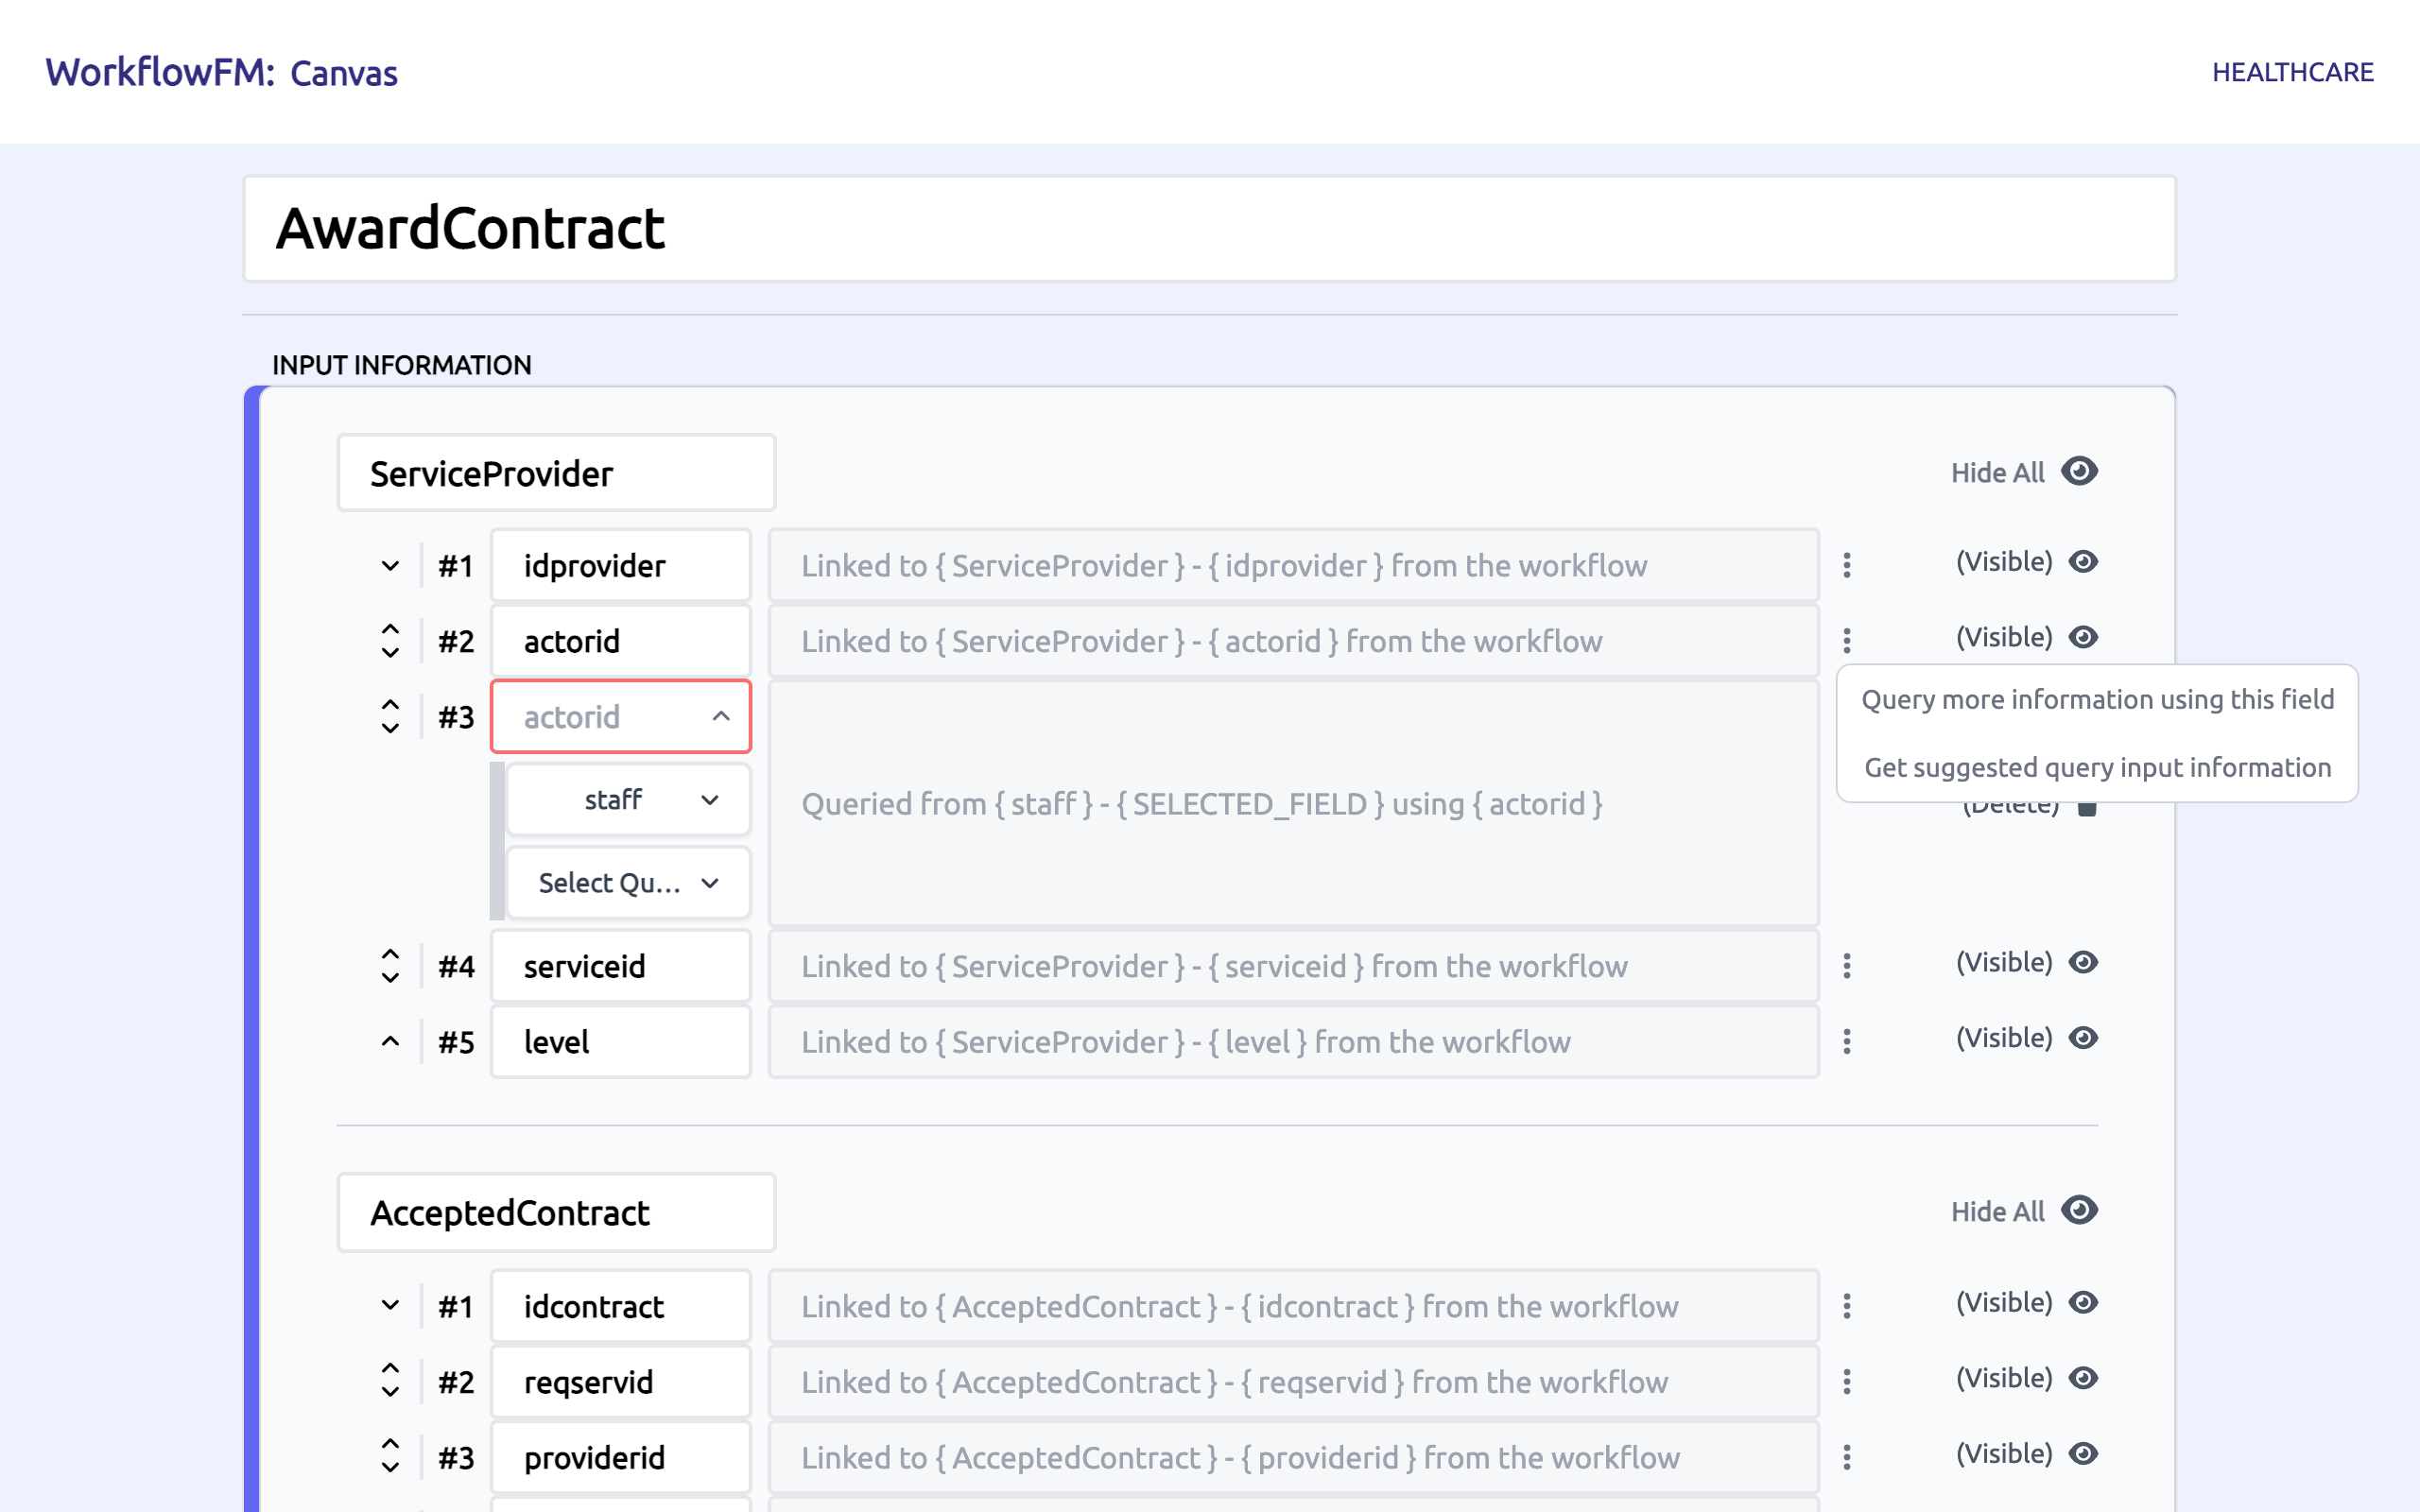
\includegraphics[width=0.9\linewidth]{overleaf/images/screens/input_information_section.png}
  \caption{Input Information Section}
  \label{fig:input_information_section}
\end{minipage}%
\begin{minipage}{.5\textwidth}
  \centering
  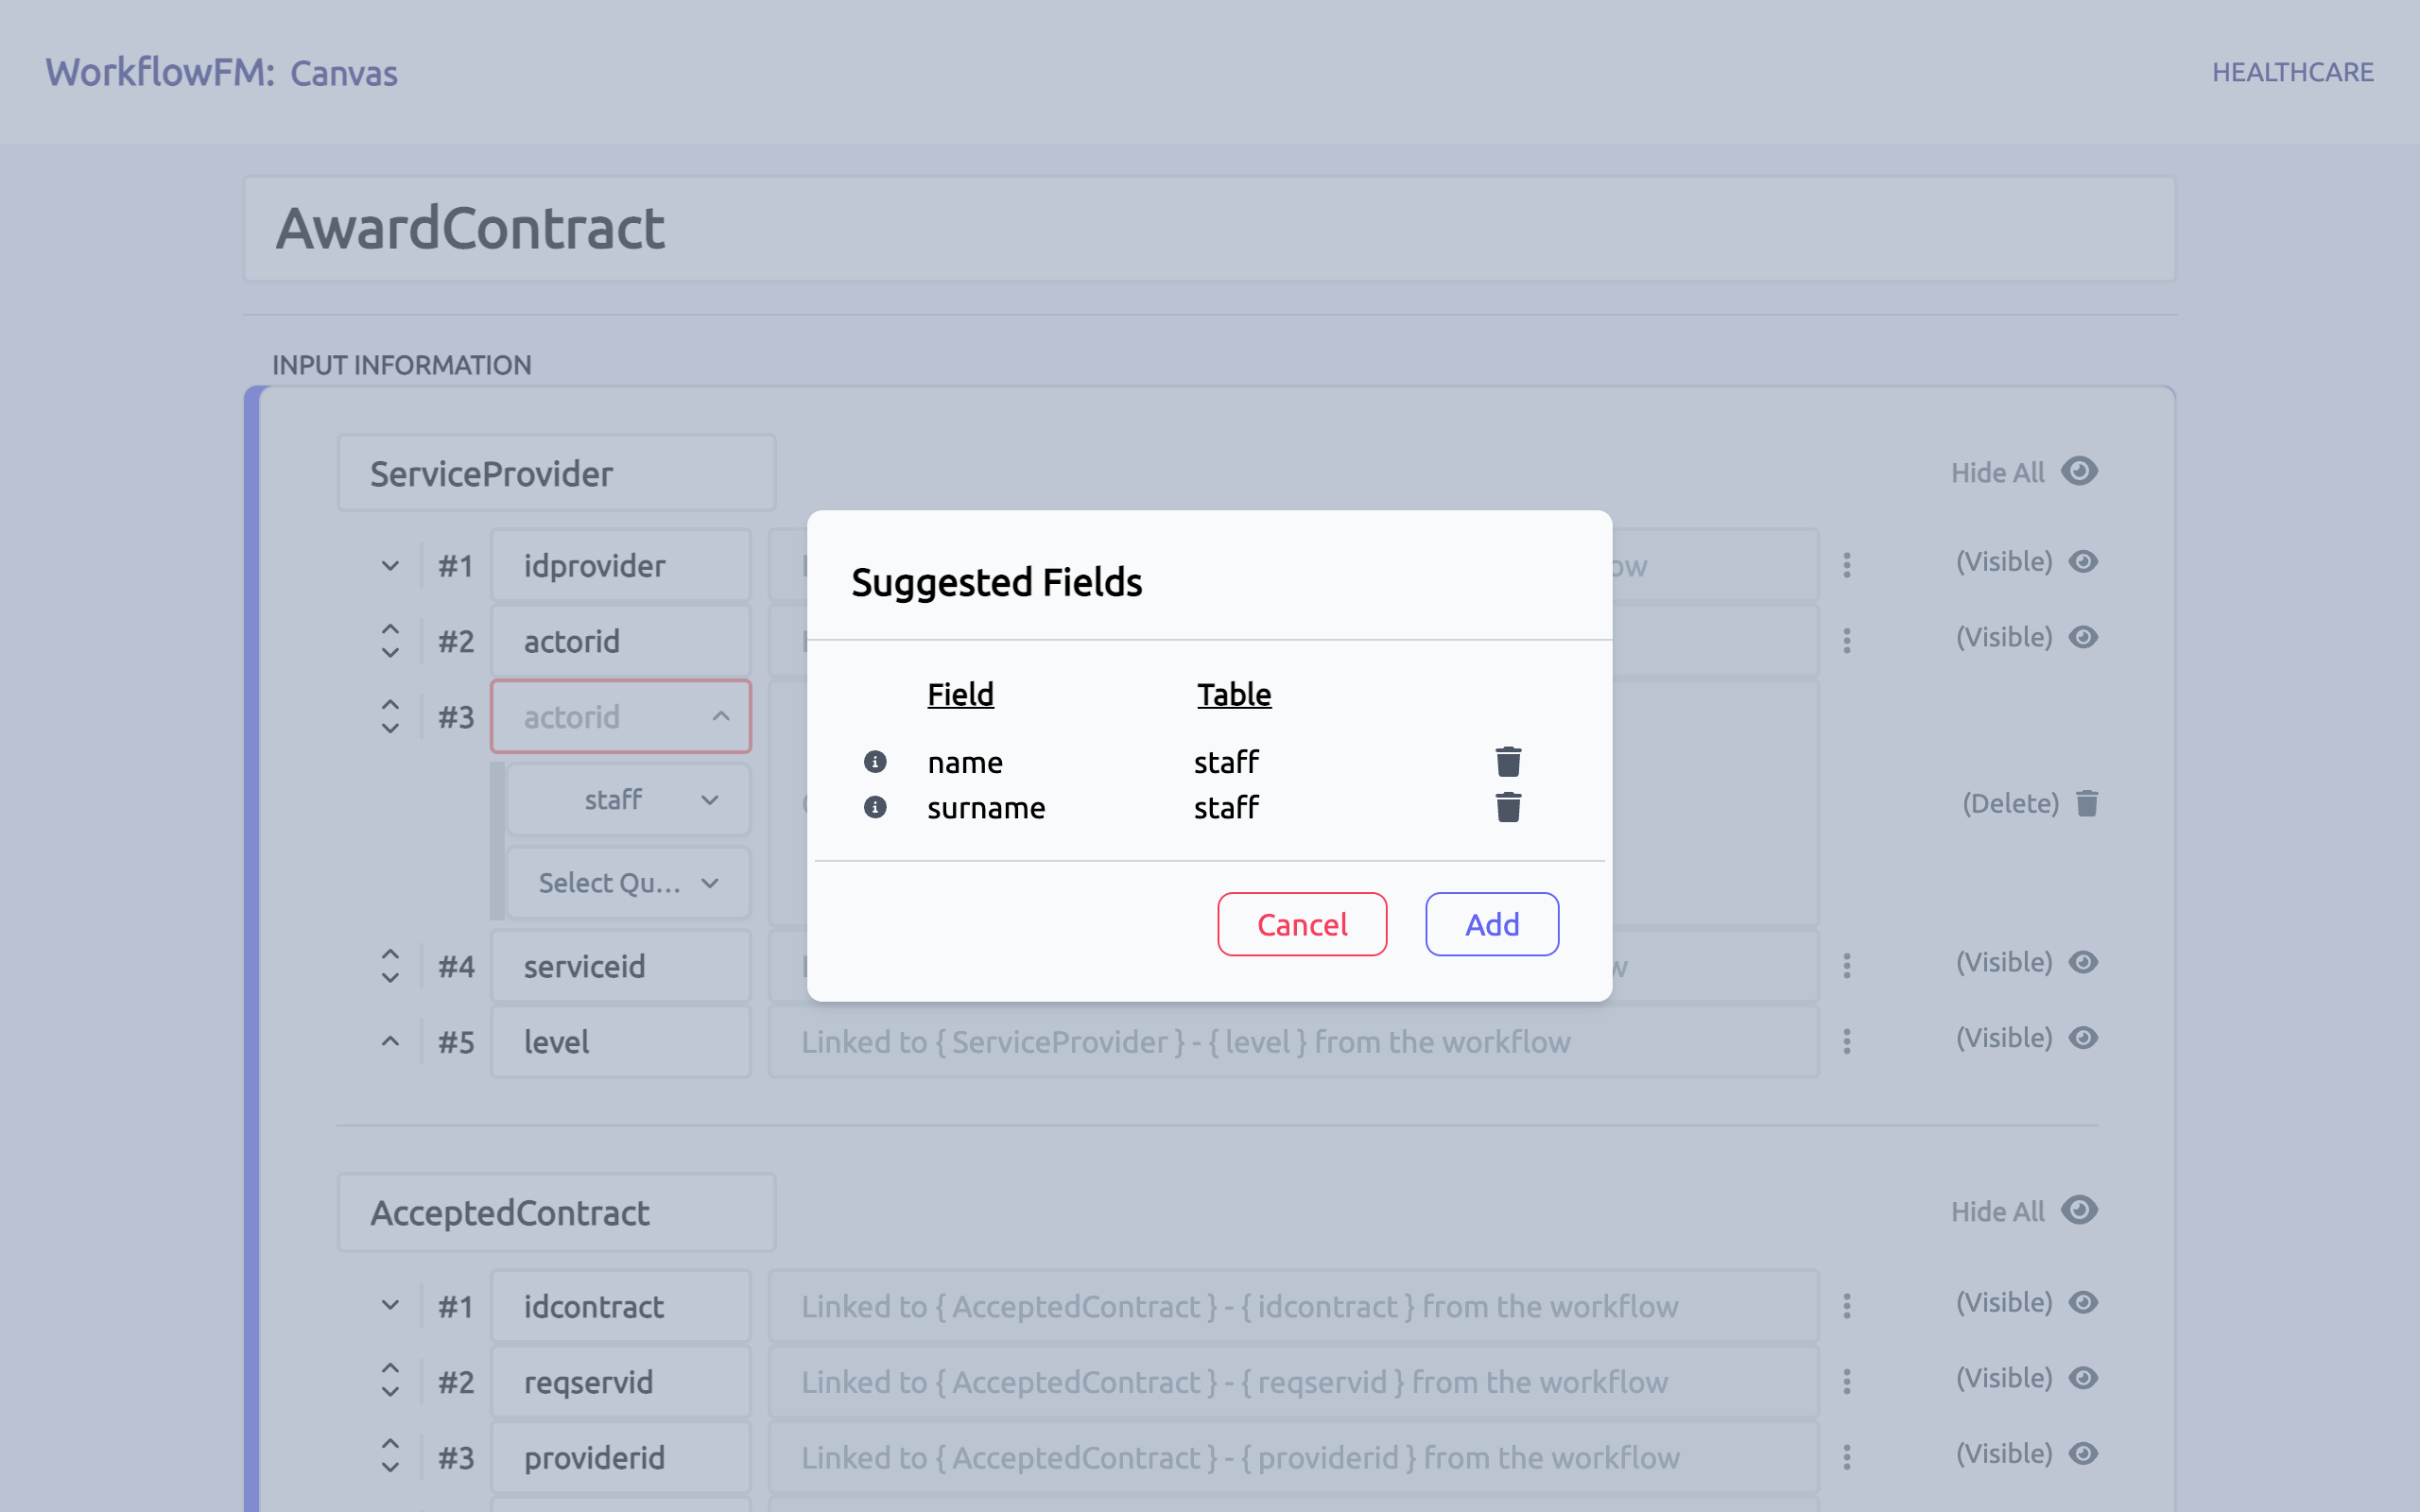
\includegraphics[width=0.9\linewidth]{overleaf/images/screens/query_suggestion.png}
  \caption{Query Suggestion Popup}
  \label{fig:query_suggestion}
\end{minipage}
\end{figure}


% \begin{figure}[ht!]
%     \centering
%     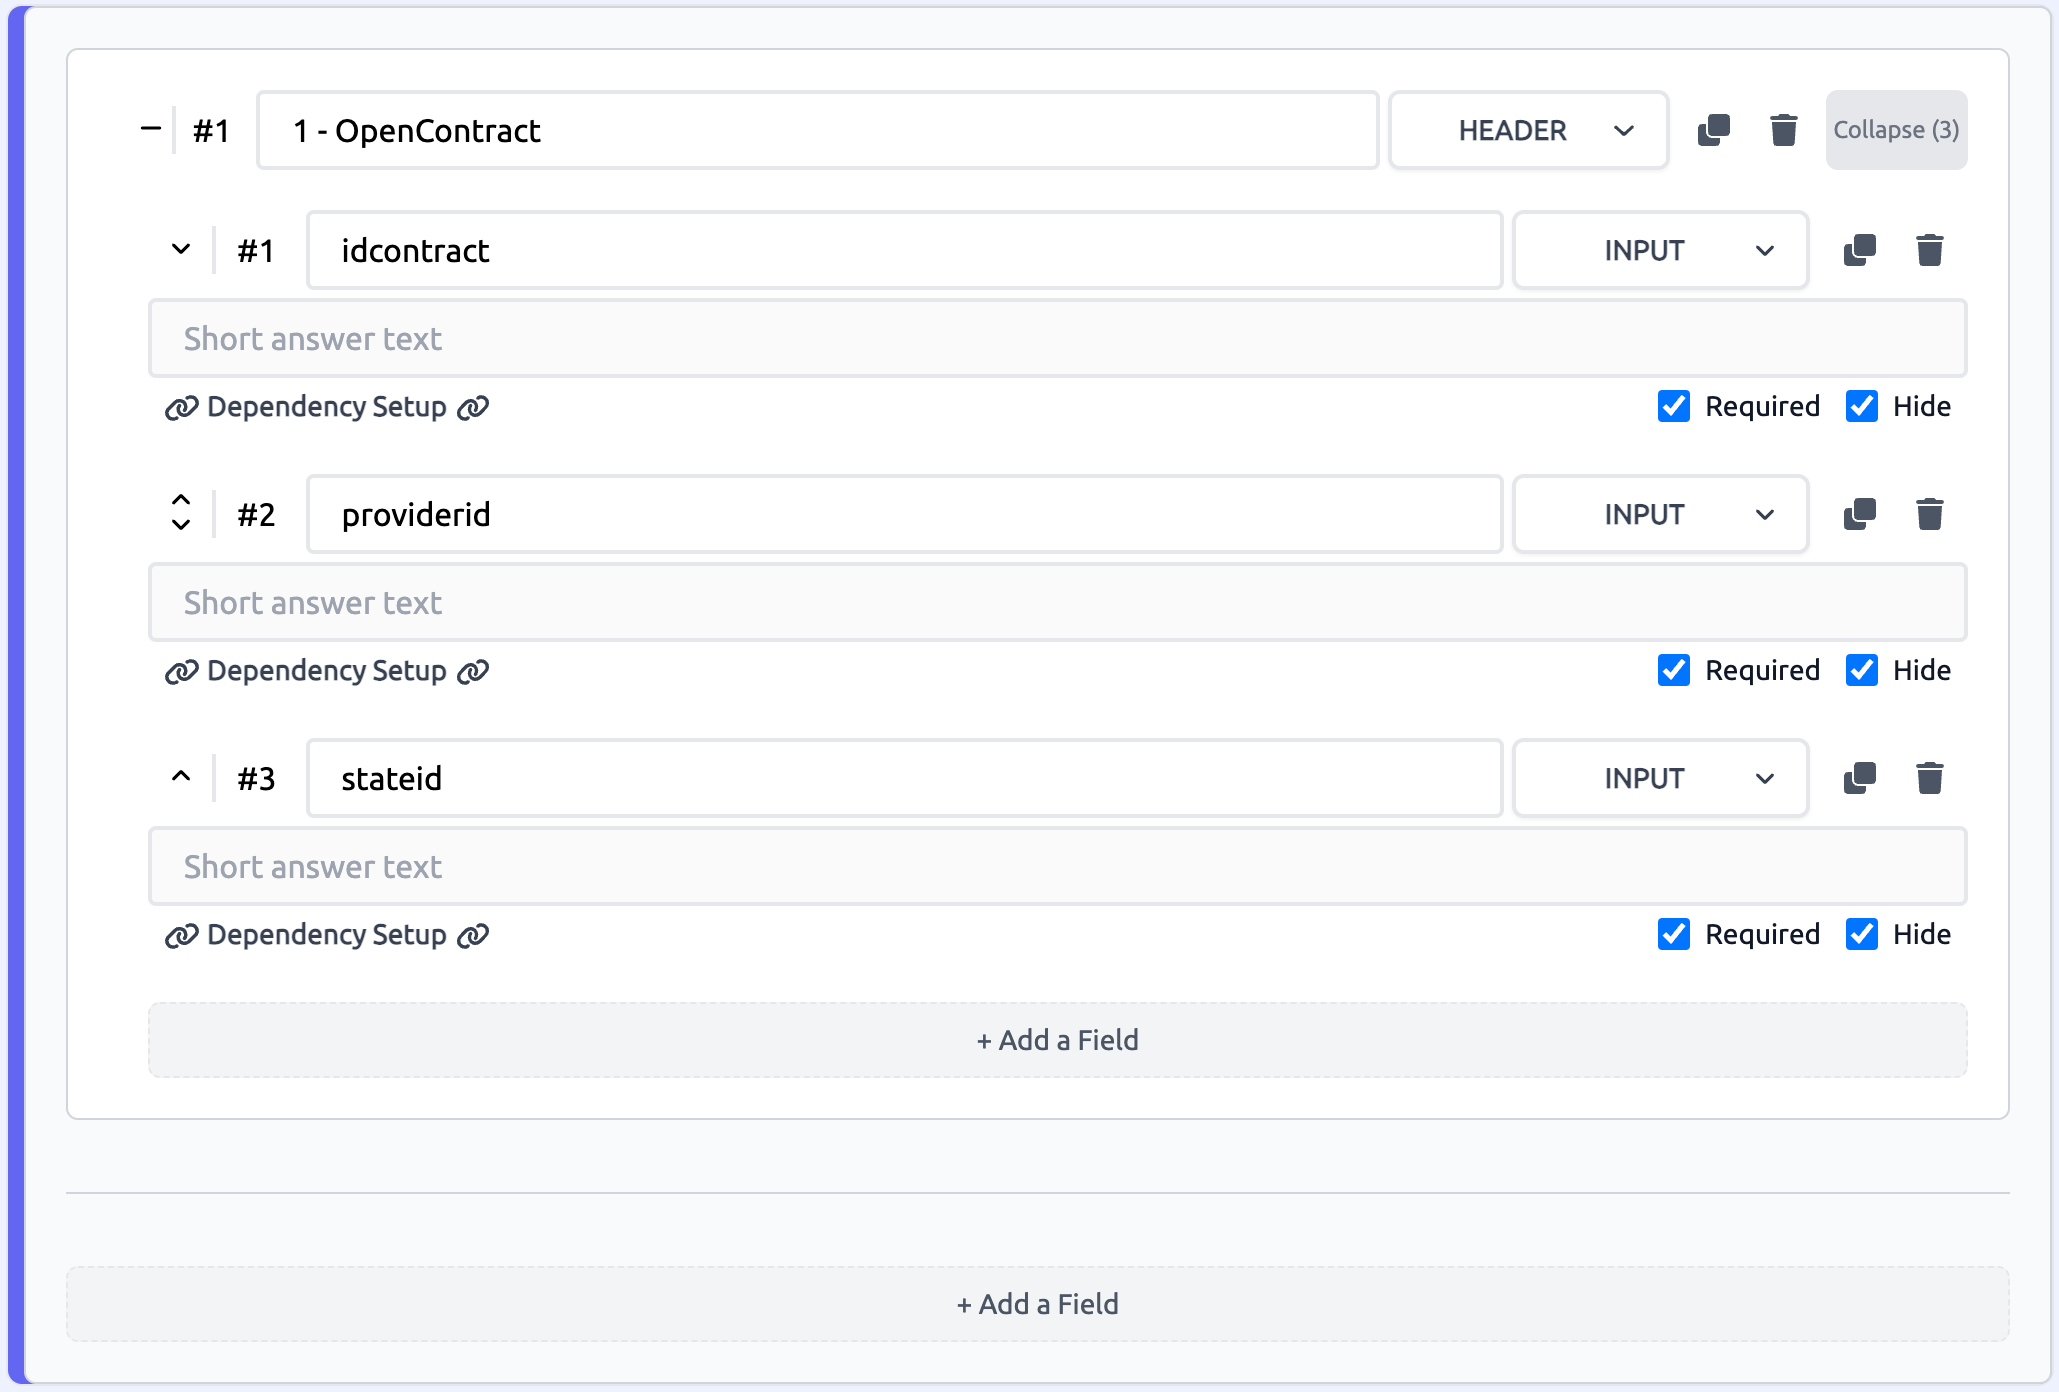
\includegraphics[width=0.5\textwidth]{overleaf/images/screens/form_section.png}
%     \caption{Form Section}
%     \label{fig:form_section}
% \end{figure}


\subsubsection{Dependencies Management Popups}
\label{im:depend_manage_pop}

Dependencies management popups can be accessed through the dependency setup button under each form component or the manage dependencies button at the bottom of the canvas screen (\ref{im:canvas_screen}). Accessing the dependency setup button will bring users to the component's dependencies setup. This popup is dedicated to each component, as shown in Figure \ref{fig:edit_dependencies_2}. On the other hand, the manage dependencies button will lead users to the all components' dependencies management popup, as seen in Figure \ref{fig:edit_dependencies}. Setting up input and output dependencies in these popups is part of the \textbf{Dependency Linking} function.

\begin{figure}[ht!]
\centering
\begin{minipage}{.5\textwidth}
  \centering
  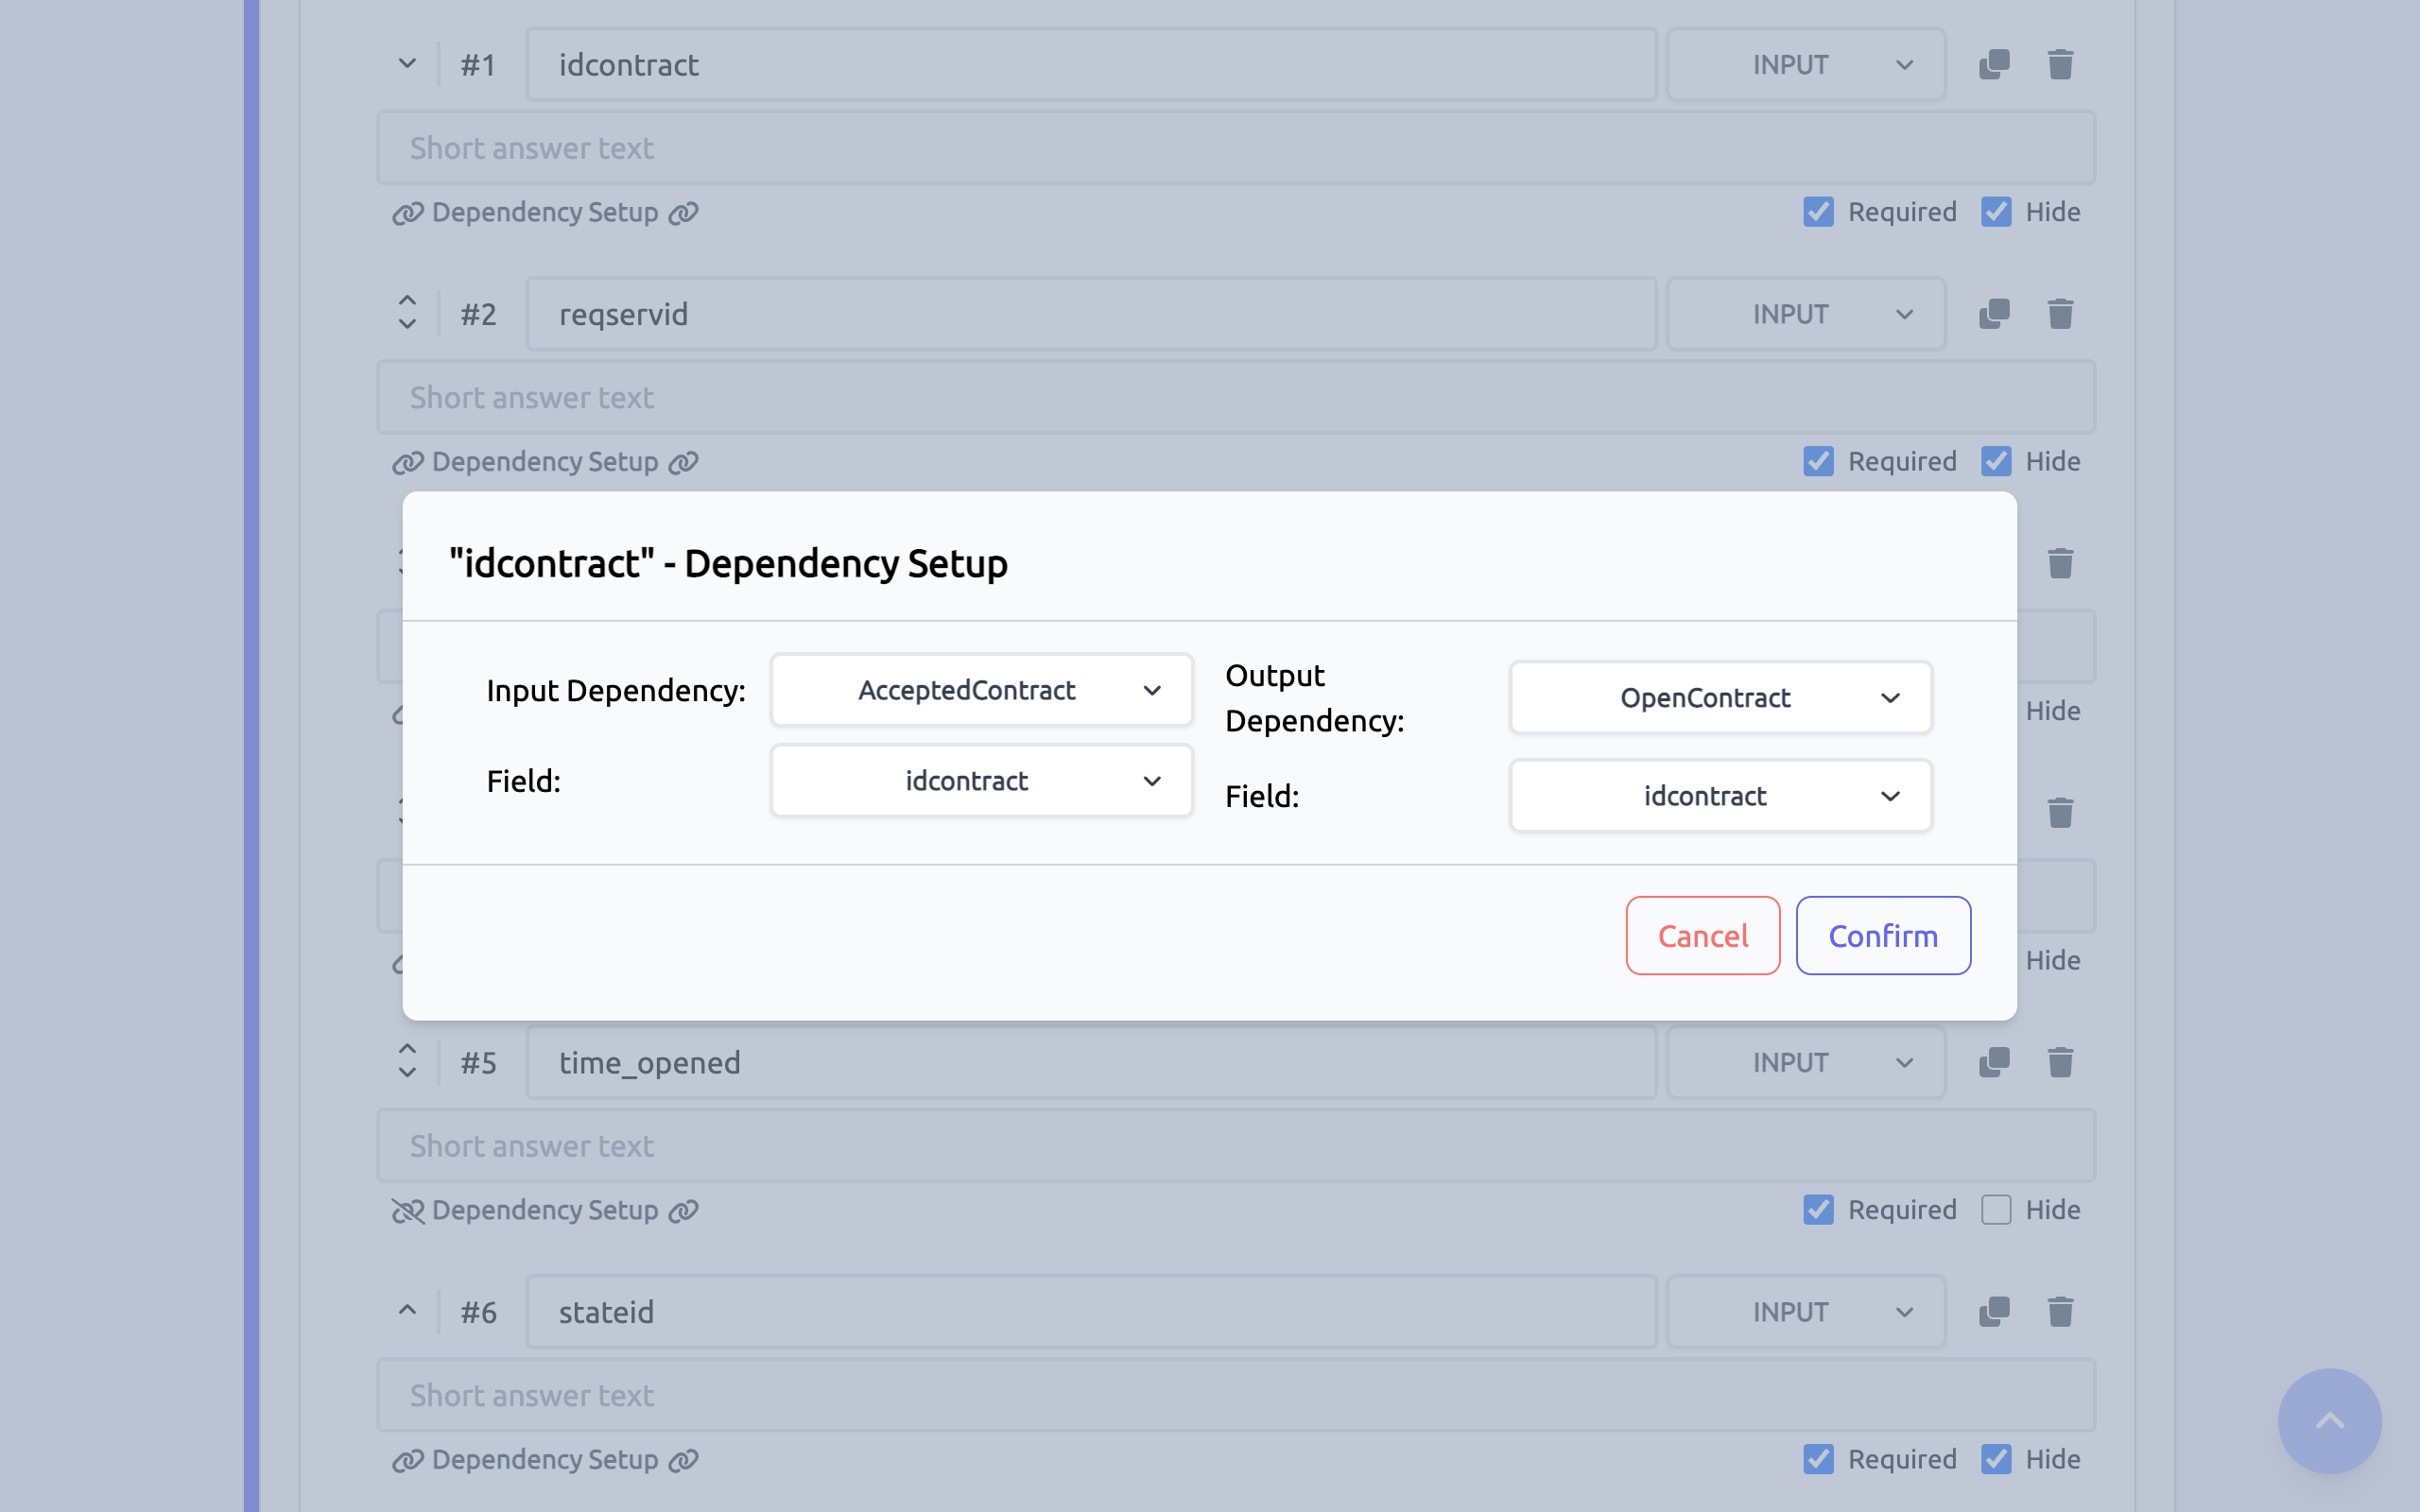
\includegraphics[width=0.9\linewidth]{overleaf/images/screens/edit_dependencies_2.png}
  \caption{Dependency Setup}
  \label{fig:edit_dependencies_2}
\end{minipage}%
\begin{minipage}{.5\textwidth}
  \centering
  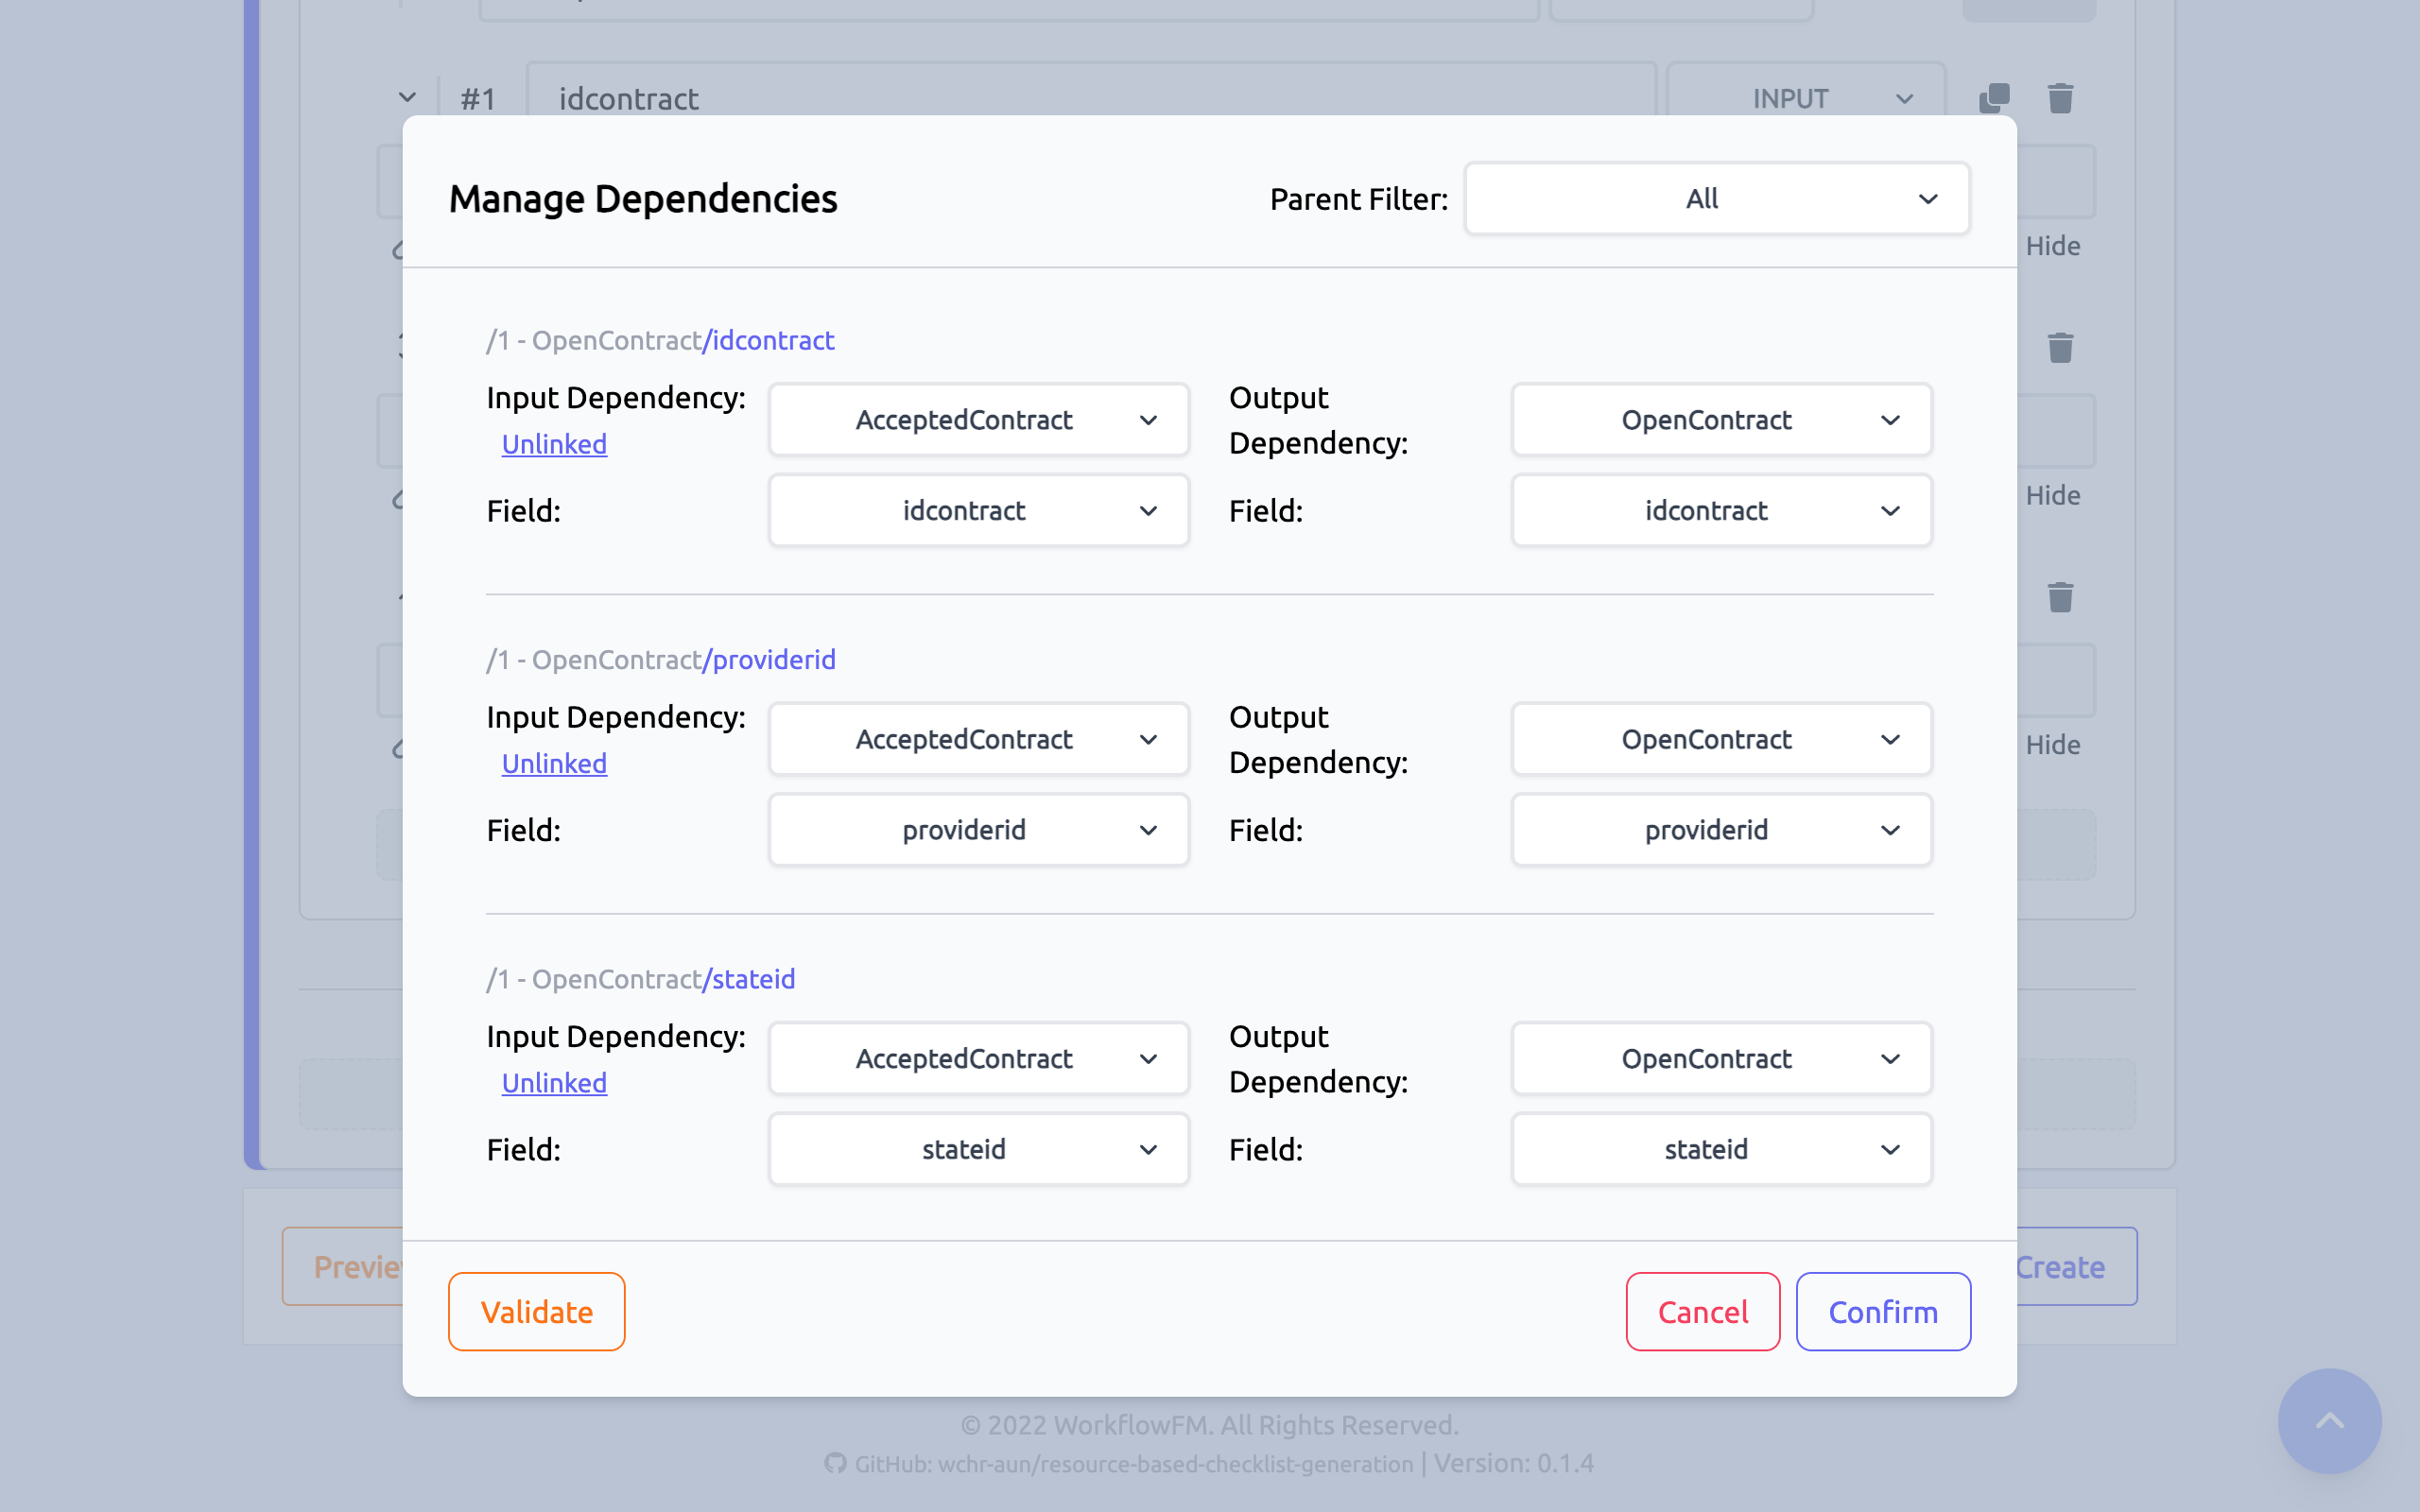
\includegraphics[width=0.9\linewidth]{overleaf/images/screens/edit_dependencies.png}
  \caption{Dependencies Management}
  \label{fig:edit_dependencies}
\end{minipage}
\end{figure}

\subsubsection{Preview Screen}
\label{im:preview_screen}

Preview screen is the screen that allows users to visualise how the template would look like when it is created. This screen can be accessed through the preview button in the canvas screen (\ref{im:canvas_screen}).

\begin{figure}[ht!]
    \centering
    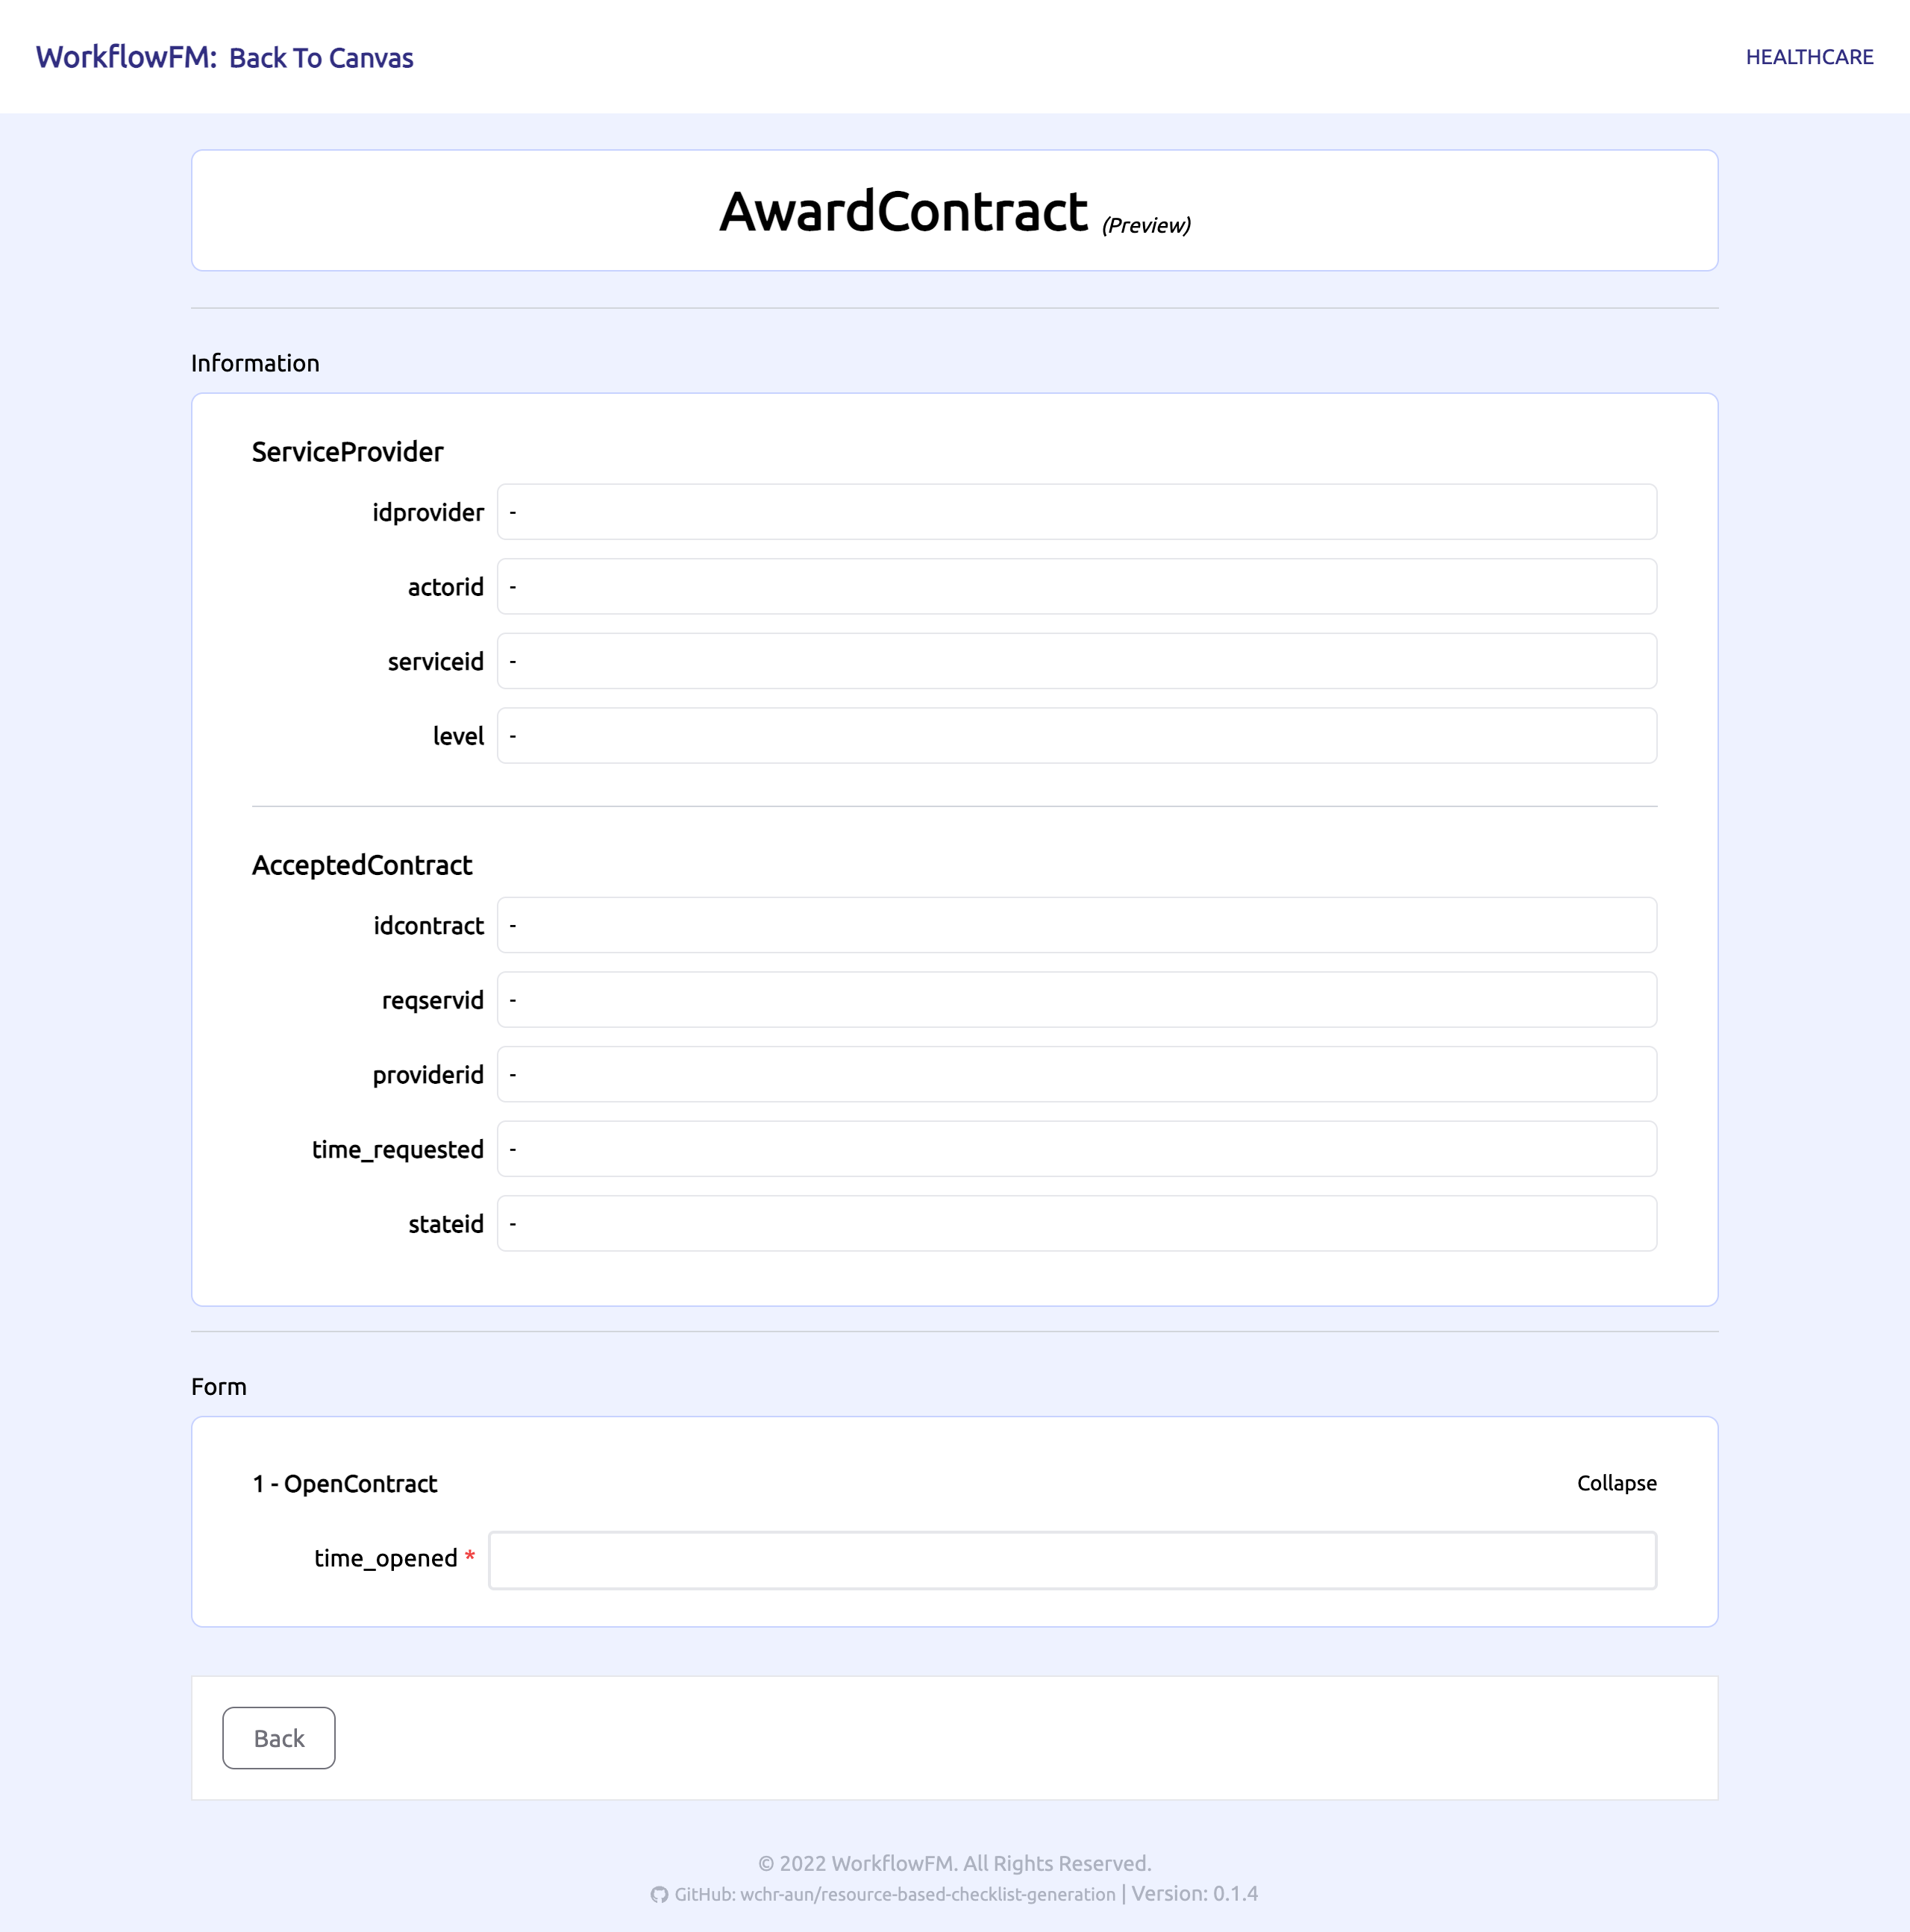
\includegraphics[width=0.55\textwidth]{overleaf/images/screens/preview_screen.png}
    \caption{Preview Screen}
    \label{fig:preview_screen}
\end{figure}





\subsection{Checklist}
\label{im:view_checklist}

As discussed in the software's structure section \ref{fig:software_structure}, this component only has one dynamic screen which displays differently based on the selected template from the list on the main screen. Being able to view a saved template is part of the \textbf{View Checklist Template} function.

\begin{figure}[ht!]
    \centering
    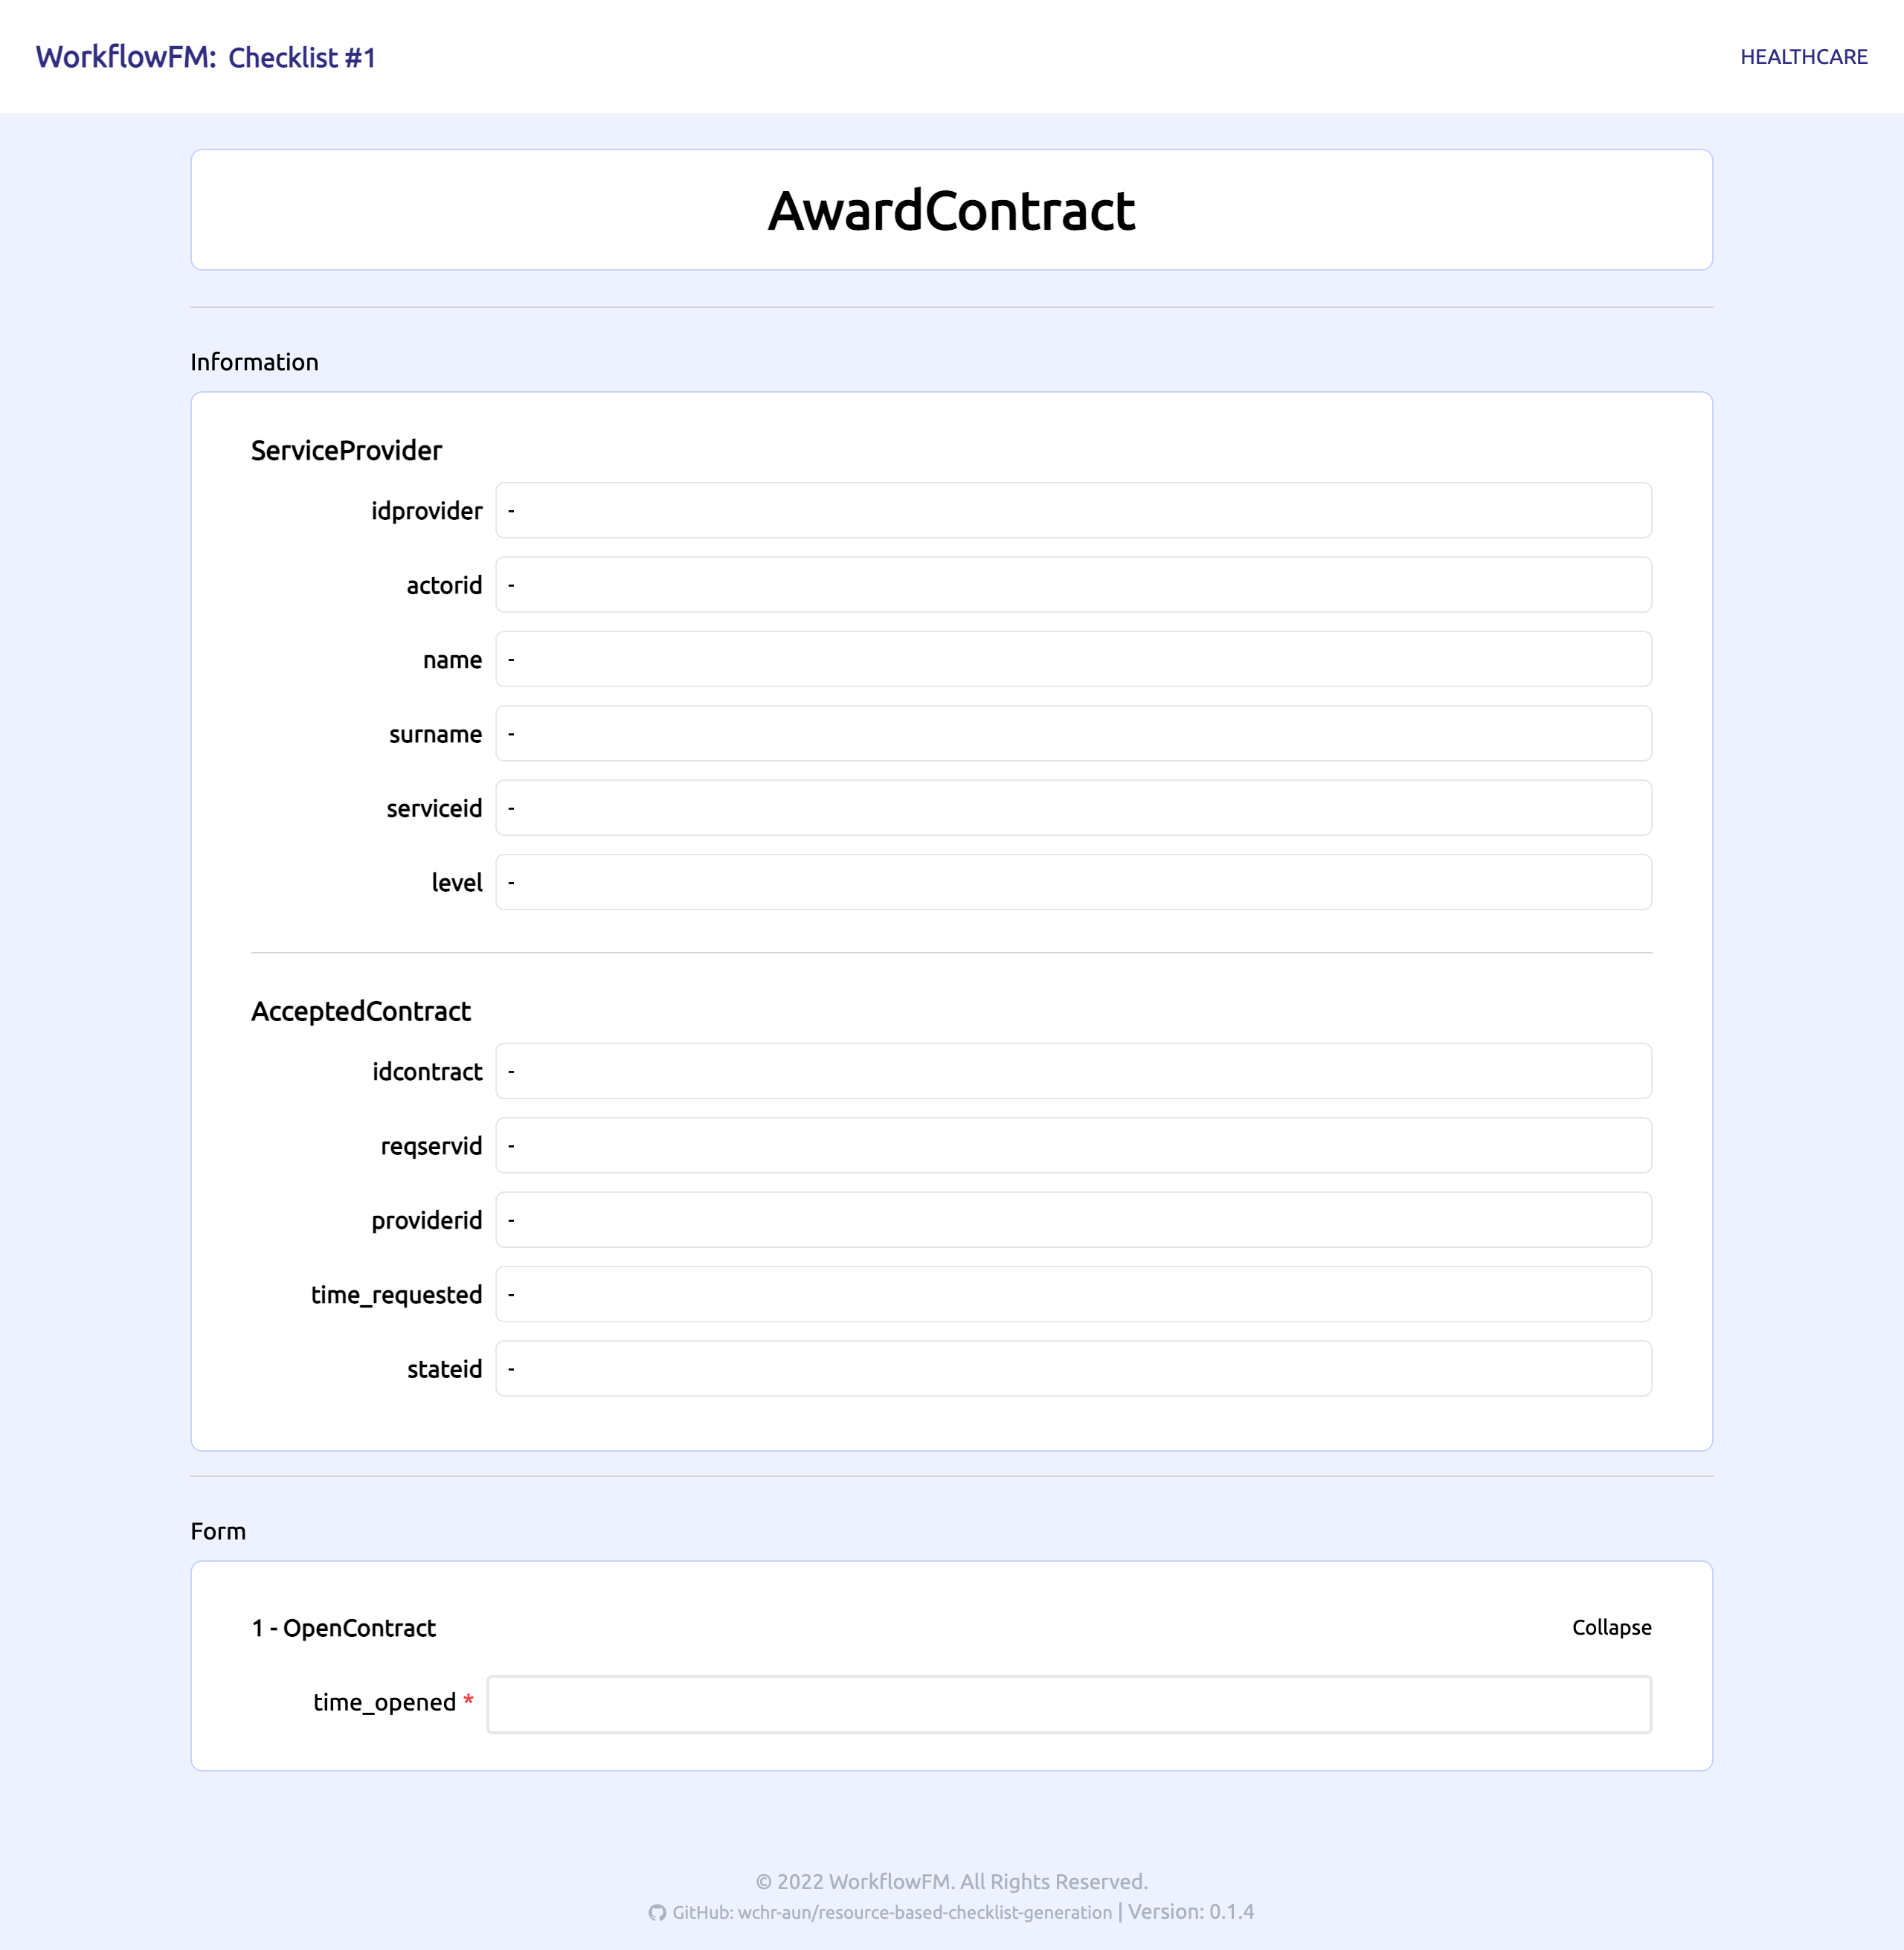
\includegraphics[width=0.55\textwidth]{overleaf/images/screens/view_checklist_screen.png}
    \caption{Checklist Screen}
    \label{fig:view_checklist_screen}
\end{figure}

\section{Backend}

asdfasd
% \subsection{Application Programming Interfaces}
% - workflow process to checklist template

% - get dependencies

% - get foreign tables/keys

% - saving template

% - retrieve finished templates


\subsection{Template}

\subsection{Dependency}
\label{backend_dependency}

\subsection{Checklist}
% \subsection{Naive Queryable Field Suggestion}
% \subsection{Naive Dependency Suggestion}


\section{Testing}


\section{Challenges}

tree structure of workflowfm's processes, doing all suggestions within sql queries, design challenges (queryable input fields)
% http4s sucks-akka-http works
